\newcommand {\LLower}[1]{\smash{\lower 3ex \hbox{#1}}}
\newcommand {\Lower}[1]{\smash{\lower 1.5ex \hbox{#1}}}
\newcommand {\SLower}[1]{\smash{\lower 0.5ex \hbox{#1}}}

\def\XX{{\cal X}}
\def\SS{{\cal S}}
\def\DD{{\cal D}}
\def\a{{\alpha}}
\def\b{{\beta}}
\def\ba{{\bm{\alpha}}}
\def\bb{{\bm{\beta}}}
\def\y{{\bf y}}
\def\I{{\bf I}}
\def\B{{\bf B}}
\def\A{{\bf A}}
\def\x{{\bf x}}
\def\K{{\bf K}}
%\def\K{K}
\def\L{{\bf L}}
%\def\L{L}
\def\S{{\bf S}}
\def\C{{\bf C}}
\def\D{{\bf D}}
\def\E{{\bf E}}
\def\P{{\bf P}}
\def\T{{\bf T}}
%\def\T{T}
\def\bsigma{\mbox{\boldmath $\sigma$}}
\def\blambda{\mbox{\boldmath $\lambda$}}
\def\bmu{\mbox{\boldmath $\mu$}}
\def\V{{\bf V}}
\def\0{{\bf 0}}
\def\1{{\bf 1}}
\def\v{{\bf v}}
\def\tr{{\mbox{tr}\;}}
\def\diag{{\mbox{diag}}}
\def\st{{\mbox{s.t.}}}
\def\psd{{\succeq\0}}
\def\pd{{\succ\0}}
\def\Z{{\bf Z}}
%\def\J{{\mathcal J}}
\def\J{J}
\def\rk{{\mbox{r}}}

\newcommand{\dataset}{{\cal D}}
\newcommand{\fracpartial}[2]{\frac{\partial #1}{\partial  #2}}


%---------------------------------------------------------------------------------
\chapter{Simple Non-Parametric Kernel Learning Algorithms}\label{chp:npkl}
%---------------------------------------------------------------------------------

%Comparing with parametric kernel learning methods, like MKL, {\em non-parametric kernel learning (NPKL)} has more flexibility to fit the data. Previous studies of NPKL usually formulate the learning task as a Semi-Definite Programming (SDP) problem that is often solved by some general purpose SDP solvers. However, for $N$ data examples, the time complexity of NPKL using a standard interior-point SDP solver could be as high as $O(N^{6.5})$, which prohibits NPKL methods applicable to real applications, even for data sets of moderate size. In this chapter, we present a family of efficient NPKL algorithms, termed ``{\bf SimpleNPKL}", which can learn non-parametric kernels from a large set of pairwise constraints efficiently. In particular, we propose two efficient SimpleNPKL algorithms. One is SimpleNPKL algorithm with linear loss,
%which enjoys a {\it closed-form} solution that can be efficiently computed by the \emph{Lanczos} sparse eigen decomposition technique. Another one is SimpleNPKL algorithm with other loss functions (including square hinge loss, hinge loss, square loss) that can be re-formulated as a saddle-point
%optimization problem, which can be further resolved by a fast iterative algorithm. In
%contrast to the previous NPKL approaches, our empirical results show that the
%proposed new technique, maintaining the same accuracy, is significantly more efficient
%and scalable. Finally, we also demonstrate that the proposed new technique is also
%applicable to speed up many kernel learning tasks, including {\it colored maximum
%variance unfolding}, {\it minimum volume embedding}, and {\it structure preserving
%embedding}. The major content of this chapter has been published by \cite{jmlr/ZhuangTH11}.

%
%Kernel methods have been successfully applied in various real applications ranging from data mining, computer vision and bioinformatics, and often show the state-of-the-art performance (refer to \cite{as/HofmannSAS08} and references therein). Empirical evidences show that the generalization performance of kernel methods is often dominated by the chosen kernel function.
%Inappropriate kernels could lead to sub-optimal or even poor results. Therefore, the choice of an effective kernel plays a crucial role in many kernel based machine learning methods. Typically, traditional kernel methods, for example, Support Vector Machines (SVMs), often adopt a predefined kernel function that is empirically chosen from a pool of parametric kernel functions, such as polynomial and Gaussian kernels. One major limitation of such an approach is that choosing an appropriate kernel function manually may require a certain level of expert knowledge, which may be difficult in some situations. Another limitation lies in the difficulty of tuning optimal parameters for the predefined parametric kernel functions.

As introduced in chapter 2, to address the problem of kernel learning, a bunch of research on learning effective kernels from data automatically has been actively explored recently. An example technique is
\emph{Multiple Kernel Learning} (MKL) \cite{jmlr/LanckrietCBGJ03,icml/BachLJ04}, which aims at learning a convex combination of several predefined parametric kernels in order to identify a good target kernel for the applications. MKL has been actively studied in many
applications, including bio-informatics \cite{nips/SonnenburgRS05,jmlr/SonnenburgRSS06}, computer vision \cite{cvpr/DuanTXM09,cvpr/SunWYCCL09,iccv/VedaldiGVZ09}, and natural language processing \cite{corr/MaoT11}, etc. Despite some encouraging results reported, these techniques often assume the target kernel function is of some {\it parametric} forms, which limits their capacity of fitting diverse patterns in real complex applications.

Instead of assuming some parametric forms for the target kernel, an emerging group of kernel learning studies are devoted to \emph{Non-Parametric Kernel Learning} (NPKL) methods, which aim to learn a Positive Semi-Definite (PSD) kernel matrix directly from the data. Example techniques include \cite{nips/CristianiniSEK01}, \cite{jmlr/LanckrietCBGJ03}, \cite{nips/ZhuKGL04}, \cite{nips/ZhangA05}, \cite{icml/KulisSD06}, \cite{icml/HoiJL07}, \cite{jmlr/KulisSD09} and \cite{aistats/LiFDSW09,uai/MaoT10}. NPKL provides a flexible learning scheme of incorporating prior/side information into the known similarity measures such that the learned kernel can exhibit better ability to characterize the data similarity. However, due to the PSD constraint, the resulting
optimization task of NPKL is often in the form of Semi-Definite Programing (SDP). Many existing studies have simply solved such SDP problems by some general purpose SDP solvers, which often have the time complexity of $O(N^{6.5})$, making the NPKL solution infeasible to real world large-scale applications.

In this chapter, we aim at addressing the efficiency and scalability issues related to the NPKL techniques proposed by \cite{icml/HoiJL07} and \cite{icml/ZhuangTH09}, which have shown the state-of-the-art empirical performance in several applications \cite{civr/ZhuangH10}. In particular, the main contributions of this chapter include:
\begin{enumerate}
\item We propose a family of Simple Non-Parametric Kernel Learning (SimpleNPKL) algorithms for efficient and scalable non-parametric kernel learning.

\item We present the first SimpleNPKL algorithm with linear loss function to learn non-parametric kernels from pairwise constraints. The algorithm enjoys a {\em closed-form} solution that can be computed efficiently by sparse eigen-decomposition techniques, for example, the \emph{Lanczos} algorithm.

\item To achieve more robust performance, we propose the second SimpleNPKL algorithm that has other loss functions (including square hinge loss, hinge loss and square loss), which can be re-formulated as a {\it mini-max optimization} problem. This optimization can be solved by an efficient iterative projection algorithm that mainly involves the computation of sparse eigen decomposition.

\item To further speed up the SimpleNPKL algorithm of other loss functions, we investigate some active constraint selection techniques to reduce the computation cost at each iteration step.

\item We conducted extensive experiments, which show that SimpleNPKL is significantly more efficient than existing NPKL methods. With the same linear loss function, SimpleNPKL is on average $40$ times faster than the original NPKL using a standard SDP solver. This makes the NPK learning techniques practical to large-scale applications.

\item We extend the proposed SimpleNPKL scheme to resolve other
non-parametric kernel learning problems, including {\em colored maximum
variance unfolding} \cite{nips/SongSBG07}, {\em minimum volume
embedding} \cite{aistats/ShawJ07}, and {\em structure preserving embedding}\cite{icml/ShawJ09}. The encouraging results show that our technique is able to speed up the existing non-parametric kernel learning solutions significantly for several real-world applications.
\end{enumerate}

The rest of this chapter is organized as follows. Section 3.1 introduces a framework of Non-parametric Kernel Learning (NPKL) from pairwise constraints proposed by \cite{icml/HoiJL07}. Section 3.2 describes our proposed SimpleNPKL algorithms, which aim to resolve the NPKL task efficiently. Section 3.3 discusses some implementation issues for developing a fast solver in practice. Section 3.4 extends our technique to speed up other kernel learning methods. Section 3.5 gives our empirical results and Section 3.6 concludes this work.

%\section{Review of Non-Parametric Kernel Learning}\label{sec:relatedwork}
%
%By simply relaxing the optimization domain $\mathcal K$, one can turn a regular kernel learning scheme to some NPKL formulations. For example,
%
%The kernel learning formulation discussed above aims to optimize both the classifier and the kernel matrix simultaneously. Some theoretical foundations, such as existence and uniqueness of the target kernel, were given in
%\cite{jmlr/MicchelliP05} and \cite{colt/ArgyriouMP05}.
%
%Another line of kernel learning research mainly focuses on optimizing the kernel only with respect to some criteria under some prior constraints or heuristics. An important technique is the kernel target alignment criterion proposed in \cite{nips/CristianiniSEK01}, which guides the kernel learning task to optimize the kernel by maximizing the alignment between the training data examples and the class labels of the training examples:
%\begin{eqnarray}
%&\max_{\K\psd}& \frac{\langle \K_{N_l}, \T \rangle} {\sqrt{\langle \K_{N_l}, \K_{N_l} \rangle \langle \T, \T\rangle}}, \label{eqn:alignment}
%\end{eqnarray}
%where $\T=\y\y'$ is the outer product of labels, $\K_{N_l}$ is the sub-matrix of which the entry values are kernel evaluation on $N_l$ labeled data examples. Note that $\T$ could be obtained by empirical experiments and more general than class labels. The objective (\ref{eqn:alignment}) only involves the labeled data. A popular assumption is to treat $\K$ to be spanned by the eigen-vectors of some known kernel defined over both the labeled and unlabeled data
%\cite{nips/ChapelleWS02,nips/ZhuKGL04,kdd/HoiLC06,nips/ZhangA05,tit/JohnsonZ08}:
%$\mathcal K=\{\sum_i\lambda_i\mathbf v\mathbf v':\lambda_i\geq 0\}$. Thus the optimization variables are reduced from the entire kernel matrix $\K$ to the kernel spectrum $\blambda$.
%
%Recently \cite{icml/HoiJL07} proposed an NPKL technique that aims to learn a fully
%non-parametric kernel matrix from pairwise constraints. The target kernel is
%maximally aligned to the constraint matrix $\T$ and minimally aligned to the graph
%Laplacian. The objective can be deemed as a form of kernel target alignment without
%normalization. Since our proposed family of SimpleNPKL algorithms follows this
%framework, we will discuss the details of this formulation in Section \ref{sec:NPK}.
%
%Besides the normalized inner product, which measures the similarity between $\K$
%and the target $\T$, researchers have also proposed dissimilarity based criteria. In
%fact, the preceding indefinite kernel learning (\ref{eqn:indefinite}) employs the
%Euclidean distance to measure the dissimilarity between kernels. Besides, another
%example in \cite{icml/KulisSD06} employed the Bregman divergence to measure
%distance between $\K$ and a known kernel $\K_0$:
%\begin{eqnarray}
%&\min_{\K\psd}& D_{\phi}(\K,\K_0)\triangleq \tr\K\K_0^{-1} - \log\det(\K\K_0^{-1}) - N, \label{eqn:bregman}
%\end{eqnarray}
%where $D_{\phi}$ is a Bregman divergence \cite{icml/KulisSD06}.
%
%The optimization over the above learning objective function (\ref{eqn:alignment}) or (\ref{eqn:bregman}) will simply return the trivial solution $\K_0$ without additional constraints, which would make NPKL meaningless. In practice, some prior knowledge about the target kernel will be added to constrain the solution space $\mathcal K$. Most of the existing constraints over the entries of $\K$ could be expressed by $\tr\K\T\leq b$. For example, as discussed in \cite{icml/Kwok03}, the square of distance between two data examples $\x_i$ and $\x_j$ in the feature space can be expressed by $\|\Phi(\x_i) - \Phi(\x_j)\|^2_2 = K_{ii} + K_{jj} - 2K_{ij} = \tr\K\T_{ij}$, where $\T_{ij}$ is a matrix of $N\times N$ only taking non-zeros at $T_{ii}=T_{jj}=1, T_{ij}=T_{ji} = -1$. Moreover, one can introduce slack variables for soft constraints.
%
%Besides, some regularization terms over kernel $\K$ are often included during the optimization phase. For example, fixing the trace $\tr\K=1$ is rather common in SDP solvers.
%
%At last, we summarize the typical schemes of existing NPKL methods:
%\vspace{-0.1in}
%\begin{itemize}
%  \item To encourage the similarity (e.g., kernel target alignment) or penalize the distance
%    (e.g., Bregman divergence) to some prior similarity information; \vspace{-0.1in}
%  \item To enforce some constraints to the kernel $\K$ with prior heuristics, such as
%    distance constraint $K_{ii}+K_{jj}-2K_{ij}=d_{ij}^2$, or side information,
%    etc; and \vspace{-0.1in}
%  \item To include regularization terms over $\K$ to control capacity, such as $\tr\K=1$.
%    \vspace{-0.1in}
%\end{itemize}
%
%By the above steps, NPKL provides a flexible scheme to incorporate more prior
%information into the target kernel. Due to the non-parametric nature, the solution
%space $\mathcal K$ is capable of fitting diverse empirical data such that the learned
%kernel $\K$ can be more effective and powerful to achieve better empirical
%performance than traditional parametric kernel functions.
%
%%\subsubsection{Optimization Aspects}
%
%Despite the powerful capacity achieved by NPKL, one key challenge with NPKL is
%the difficulty of the resulting optimization problem, in which \vspace{-0.1in}
%\begin{itemize}
%  \item the whole gram matrix $\K$ is treated as the optimization variable, that is,
%    $O(N^2)$ variables; \vspace{-0.1in}
%  \item the kernel matrix $\K$ must be positive semi-definite. \vspace{-0.1in}
%\end{itemize}
%As a result, NPKL is often turned into a Semi-Definite Programming (SDP) problem. For instance, a NPKL problem to learn a kernel matrix $\K$ with $m$ linear constraints is written as follows:
%\begin{eqnarray}
%\max_{\K \psd} \tr \C\K \;\;\;:\;\;\; \tr\T_{ij}\K = b_{ij}, \label{eq:SDP_dual}
%\end{eqnarray}
%where $\C$ and $\T_{ij}$'s are $N\times N$ symmetric matrices and $b_{ij}$'s are scalars, and its dual problem can be rewritten as:
%\begin{eqnarray}
%\min_{\y} \mathbf b'\y \;\;\;:\;\;\; \C-\sum_{(i,j)}\T_{ij}y_{ij} \psd, \label{eq:SDP_primal}
%\end{eqnarray}
%where $\y$ is the vector of dual variables $y_{ij}$'s for the linear constraints in (\ref{eq:SDP_dual}) and $\mathbf b$ is the vector of $b_{ij}$'s.
%
%Typically, this SDP problem of NPKL is usually solved by applying a general
%purpose SDP solver. Among various SDP solvers, the {\em interior-point algorithm} is one of the state-of-the-art solutions~\cite{Boyd}. From \cite{laa/LoboVBL98}, the time complexity per iteration of the SDP problem (\ref{eq:SDP_primal}) is $O(m^2N^2)$. Using the primal-dual method for solving this SDP, the
%accuracy of a given solution can be improved by an absolute
%constant factor in $O(\sqrt{N})$ iterations \cite{NesterovN94}. When $m$ approaches to $O(N^2)$, the overall computation complexity is often as high as $O(N^{6.5})$, which makes NPKL inapplicable to real applications.
%
%In this work, we focus on solving the efficiency and scalability issues of
%NPKL \cite{icml/ZhuangTH09}. In particular, we propose a family of efficient
%SimpleNPKL algorithms that can solve large-scale NPKL problems efficiently.
%Moreover, we also show that the proposed algorithms are rather general, which can
%be easily extended to solving other kernel learning applications, including
%dimensionality reduction and data embedding applications.

\section{Non-Parametric Kernel Learning from Pairwise Constraints}
\label{sec:NPK}

In this Section, we introduce the framework of Non-Parametric Kernel Learning
(NPKL) \cite{icml/HoiJL07,icml/ZhuangTH09}, which aims to learn
non-parametric kernels from side information, which  is presented in a collection of
must-link and cannot-link pairs.

\subsection{Side / Label Information}

Let $\mathcal{U} = \{\mathbf{x}_1, \mathbf{x}_2, \ldots, \mathbf{x}_N\}$ denote
the entire data collection, where each data point $\mathbf{x}_i \in \XX$. Consider a
set of $N_l$ labeled data examples,
$\mathcal{L}=\{(\mathbf{x}_1,y_1)\ldots,(\mathbf{x}_{N_l},y_{N_l})\}$, one can
use $y_iy_j$ as the similarity measurement for any two patterns $\x_i$ and $\x_j$.
Sometimes, it is possible that the class label information is not readily available, while
it is easier to obtain a collection of similar (positive) pairwise constraints
$\mathcal{S}$ (known as ``must-links", that is, the data pairs share the same class) and a
collection of dissimilar (negative) pairwise constraints $\mathcal{D}$ (known as
``cannot-links", that is, the data pairs have different classes). These pairwise constraints
are often referred to as \emph{side information}.

In general, kernel learning with labeled data can be viewed as a special case of kernel
learning with side information  \cite{icml/Kwok03,icml/KulisSD06,icml/HoiJL07},
that is, one can construct the sets of pairwise constraints $\mathcal{S}$ and
$\mathcal{D}$ from $\mathcal{L}$. In real applications, it is often easier to detect
pairwise constraint while the class label is difficult to obtain. For example, in
bioinformatics, the interaction between two proteins can be identified by empirical
experiments. These interactions are expressed naturally by pairwise constraints.
However, it could be very difficult to judge the protein function, which corresponds
to class labels. In the sequel, we focus on learning kernels from pairwise constraints.

Given $\mathcal{S}$ and $\mathcal{D}$, we construct a similarity matrix $\T \in
\mathbb{R}^{N\times N}$ to represent the pairwise constraints, that is,
\begin{eqnarray}\label{eqn:side_info}
T_{ij} = \left\{
\begin{array}{cl}
+1 & (\mathbf{x}_i, \mathbf{x}_j) \in \mathcal{S} \\
-1 & (\mathbf{x}_i, \mathbf{x}_j) \in \mathcal{D} \\
0 & \mbox{otherwise.}
\end{array}
\right.
\end{eqnarray}
A straightforward and intuitive principle for kernel learning is that the kernel entry $K_{ij}$ should be
aligned with the side information $T_{ij}$ as much as
possible \cite{nips/CristianiniSEK01}, that is, the alignment $T_{ij}K_{ij}$ of each
kernel entry is maximized.

\subsection{Locality Preserving Regularization}\label{sec:laplace}

In addition to side/label information, preserving the intrinsic geometric structure of
the data have also been explored to improve the performance of kernel learning.
Typically, most existing kernel learning
approaches \cite{icml/KulisSD06,icml/HoiJL07,icml/HoiJ08} adopt the low dimensional data
manifold \cite{icml/SindhwaniNB05} for preserving the locality of the data in
kernel learning. The following reviews an approach for exploring low dimensional data manifold in
kernel learning \cite{icml/HoiJL07}.

Let us denote by $f(\mathbf{x}, \mathbf{x}')$ a similarity function that measures the
similarity between any two data points $\x_i$ and $\x_j$, and $\S \in
\mathbb{R}^{N\times N}$ is a similarity matrix where each element $S_{ij} =
f(\mathbf{x}_i, \mathbf{x}_j)\geq 0$. Note that $f(\cdot, \cdot)$ does not have to be
a kernel function that satisfies the Mercer's condition. For a given $N$ data examples, a kernel matrix $\K$
 can be expressed as $\K=\V'\V\psd$, where
$\V=[\v_1,\ldots,\v_N]$ is the matrix of the embedding of the $N$ data examples.
The regularizer of the kernel matrix $\K$, which captures the local dependency
between the embedding of $\v_i$ and $\v_j$ (i.e., the low dimensional embedding of similar data examples should be similar w.r.t. the similarity $S_{ij}$),
can be
defined as:
\begin{eqnarray}
\Omega(\V, \S)&=& \frac{1}{2}\sum_{i,j=1}^N {S_{ij}}
\left\|\frac{\mathbf{v}_i}{\sqrt{D_i}} - \frac{\mathbf{v}_j}{\sqrt{D_j}}\right\|_2^2\nonumber\\
&=&\tr(\V\L\V^{'})=\tr(\L\K),\label{eqn:reg}
\end{eqnarray}
where $\L$ is the graph Laplacian matrix defined as:
\begin{eqnarray}\label{eqn:laplace}
\L  =  \I - \D^{-1/2}\S\D^{-1/2},
\end{eqnarray}
where $\D = \mbox{diag}(D_1, D_2, \ldots, D_N)$ is a diagonal matrix with the
diagonal elements defined as $D_i = \sum_{j=1}^N S_{ij}$.


\subsection{Formulation of Non-Parametric Kernel Learning}

Taking into consideration of both the side
information in (\ref{eqn:side_info}) and the regularizer in (\ref{eqn:reg}), the NPKL
problem is then  formulated into the {\em loss + regularization} framework \cite{icml/HoiJL07} as
follows:
\begin{eqnarray}
\min_{\K\psd} & \tr \L\K  + C\sum_{(i,j) \in (\SS\cup\DD)}\ell\big(T_{ij}K_{ij}\big),
\label{eqn:ori-npk-obj}
\end{eqnarray}
which generally belongs to a Semi-Definite Programming (SDP)
problem \cite{Boyd}. Here, $C>0$ is a tradeoff parameter to control the
empirical loss\footnote{The common choice of the loss function $\ell(\cdot)$ can be
hinge loss, square hinge loss or linear loss. } $\ell(\cdot)$ of the alignment
$T_{ij}K_{ij}$ of the target kernel and the dependency among data examples with
respect to the intrinsic data structure.

\section{SimpleNPKL: Simple Non-Parametric Kernel Learning}
\label{sec:simpleNPKL}

In this Section, we present a family of efficient algorithms for solving the NPKL
problem in (\ref{eqn:ori-npk-obj}). We refer to the proposed efficient algorithms as
``SimpleNPKL" for short.

\subsection{Regularization on $\K$}

As aforementioned, the solution space of NPKL has been relaxed to boost its flexibility and capacity of fitting diverse patterns. However, arbitrarily relaxing the solution space $\mathcal K$ could result in  over-fitting. To alleviate this problem, we introduce a regularization term:
\begin{eqnarray}
\tr(\K^p), \label{eqn:capacity}
\end{eqnarray}
where $p\geq 1$ is a parameter to regulate the capacity of $\K$. Similar
regularization terms on $\K$ have also been  adopted in previous kernel learning
studies. For example, \cite{nips/CristianiniSEK01} used $\|\K\|_F=\sqrt{\langle \K,
\K \rangle}=\sqrt{\tr(\K^2)}$ in the objective to penalize the complexity of $\K$;
while \cite{jmlr/LanckrietCBGJ03} proposed to adopt a hard constraint $\tr(\K)\leq
B$, where $B>0$ a constant, to control the capacity of $\K$.


We refer  the modified NPK learning problem with the regularization term
(\ref{eqn:capacity}) either in the objective or in the constraint to as Simple
Non-Parametric Kernel Learning (SimpleNPKL), which can be solved efficiently
without engaging any standard SDP solvers. Next we present two SimpleNPKL
algorithms that adopt several different types of loss functions.

\subsection{SimpleNPKL with Linear Loss}

First of all, we consider a linear loss function $\ell(f)=-f$, and rewrite the formulation of
(\ref{eqn:ori-npk-obj}) as the SimpleNPKL formulation:
\begin{eqnarray}
\min_{\K} \tr\left(\Bigg(\L - C\sum_{(i,j) \in (\SS\cup\DD)}
\T_{ij}\Bigg)\K\right)\;:\;\K\psd,\; \tr\K^p \!\leq\!B,
\label{eqn:npk-lin}
\end{eqnarray}
where  $\T_{ij}$ is the matrix of setting the $(i,j)$-th entry to $T_{ij}$ and other
entries to 0. To solve this problem, we first present a proposition below.

\begin{prop}\label{prop:sdp-eigen_decom}
Given $\A$ is any symmetric matrix such that $\A=\P\diag(\bsigma)\P'$, where $\P$
contains columns of orthonormal eigenvectors of $\A$ and $\bsigma$ is a vector of the
corresponding eigenvalues, and $B$ is any positive constant, the optimal solution
$\K^*$ to the following SDP problem for $p > 1$:
\begin{eqnarray}\label{eqn:AB-sdp}
\max_{\K}\tr \A\K\;\;:\;\;\K\psd,\;\;\tr\K^p \leq B,
\end{eqnarray}
can be expressed as the following closed-form solution:
\begin{equation}
\K^*=\left(\frac{B}{\tr\A_+^{\frac{p}{p-1}}}\right)^{\frac{1}{p}}\A_+^{\frac{1}{p-1}}\label{eqn:optimal_K}
\end{equation}
where  $\A_+=\P\diag(\bsigma_+)\P'$,  and $\bsigma_+$ is a vector with entries equal to $\max(0,[\bsigma]_i)$.

For $p=1$,  the optimal solution $\K^*$ can be expressed as the following
closed-form solution:
\begin{equation}
\K^*=B\A_1\nonumber%\label{eqn:optimal_K2}
\end{equation}
where  $\A_1=\P\diag(\bsigma_1)\P'$,  and $\bsigma_1$ is a vector with entries equal
to $\frac{1}{\sum_{i:[\bsigma]_i=\max_i[\bsigma]_i}1}$ for all $i$ that
$[\bsigma]_i=\max_i[\bsigma]_i$; otherwise, the entries are zeros.
\end{prop}

\begin{proof}
By introducing a dual variable $\gamma\geq 0$ for the constraint
$\tr\K^p\leq B$, and $\Z\in\mathcal S_+^n$ ($\mathcal S_+^n$ is
self-dual) for the constraint $\K\succeq \0$, we have the Lagrangian of (\ref{eqn:AB-sdp}):
\begin{equation}
{\cal L}(\K;\gamma,\Z)= \tr \A\K+\gamma(B-\tr\K^p)+\tr\K \Z.\nonumber
\end{equation}
By the Karush-Kuhn-Tucker (KKT) conditions, we have:
\begin{eqnarray}
\A-\gamma p \K^{p-1}+\Z=\0 &\mbox{ and }&
\tr\K \Z=0.\nonumber
\end{eqnarray}

First, we show that $\tr(\K\Z)=0$ is equivalent to $\K\Z=\Z\K=\0$. Since $\K\psd,
\Z\psd$, we have $\tr(\K\Z)=\tr(\K^{1/2}\K^{1/2}\Z^{1/2}\Z^{1/2})
=\|\K^{1/2}\Z^{1/2}\|_F^2.$ Thus, $\tr(\K\Z)=0$ follows that
$\K^{1/2}\Z^{1/2}=\0$. Pre-multiplying by $\K^{1/2}$ and post-multiplying by
$\Z^{1/2}$ yields $\K\Z=\0$, which in turn implies $\K\Z=\0=(\K\Z)'=\Z\K$. Hence,
$\K$ and $\Z$ can be simultaneously diagonalized by the same set of orthonormal
eigenvectors \cite{mp/AlizadehHO97}. From the first KKT condition we have $\A
=\gamma p \K^{p-1} - \Z$. Consequently, $\A$ can also be diagonalized with the
same eigenvectors as $\K$ and $\Z$.

Assume $\A=\P\diag(\bsigma)\P'$, where $\P$ contains columns of
orthonormal eigenvectors of $\A$,  and $\bsigma$ is the vector of the
corresponding eigenvalues. Then, $\K=\P\diag(\blambda)\P'$ and $\Z=\P\diag(\bmu)\P'$, where
$\blambda\geq \0$ and $\bmu \geq \0$ denote the vector of the eigenvalues of $\K$ and $\Z$ respectively. Therefore, we have
\begin{eqnarray}
\tr\K^p &=&\|\blambda\|_p^p\leq B,\label{eq:ctr}\\
\tr \A\K &=&\blambda'\bsigma,\label{eq:obj}\\
\bsigma&=&\gamma p\blambda^{p-1}-\bmu,\label{eq:kkt1}\\
\blambda'\bmu&=&0 \label{eq:kkt2} .
\end{eqnarray}
Together with $\blambda\geq \0$ and $\bmu\geq \0$, and from (\ref{eq:kkt2}),
$[\blambda]_i$ and $[\bmu]_i$ cannot be both non-zeros. Hence, from (\ref{eq:kkt1}), we
know $\bsigma_+=\gamma p\blambda^{p-1}$ contains all positive components of $\bsigma$. Moreover, from  (\ref{eq:obj}) and $\blambda \geq \0$, together with the constraint
(\ref{eq:ctr}), the SDP problem
(\ref{eqn:AB-sdp}) is reduced to
\begin{eqnarray}
\max_{\blambda} \blambda'\bsigma_+ \;\; : \;\; \|\blambda\|_p^p \leq B.\nonumber
\end{eqnarray}
By H\"{o}lder inequality, we have
$\blambda'\bsigma_+ \leq \| \blambda \|_p \| \bsigma_+ \|_q$, where it holds for $1 / p + 1 / q = 1$. The equality is achieved if and only if
$|\blambda|^p$ and $|\bsigma_+|^q$ are linearly dependent. Thus we can scale $\K$ satisfying
(\ref{eq:ctr}) to arrive at the closed-form solution of $\K$ in (\ref{eqn:optimal_K})
for $p>1$.

For $p = 1$, from Equations (\ref{eq:ctr}) and (\ref{eq:obj}), the optimization task is
simplified as $\max \blambda'\bsigma :\blambda\geq 0,\| \blambda \|_1 \leq B$. Due to
the linearity, the maximum objective value is obtained by choosing $[\blambda]_i =
B/\sum_{i:[\bsigma]_i=\max_i[\bsigma]_i}1$ for all $i$ that $[\bsigma]_i = \max_i
[\bsigma]_i$; otherwise, $[\blambda]_i = 0$.
\end{proof}

Based on Proposition~\ref{prop:sdp-eigen_decom}, we can easily solve the
SimpleNPKL problem. In particular, by setting $\A=C\sum_{(i,j) \in
(\SS\cup\DD)}\T_{ij}-\L$, we can directly compute the optimal $\K^*$ to
SimpleNPKL of (\ref{eqn:npk-lin}) using sparse eigen-decomposition as in
(\ref{eqn:optimal_K}). Thus the computation cost of SimpleNPKL with linear loss is
dominated by eigen-decomposition. It is clear that this can significantly reduce the
time cost for the NPKL tasks. Alternatively, we  add $\tr(\K^p)$ directly into the
objective, and arrive at the following formulation:
\begin{eqnarray}
\min_{\K} \tr\left(\Bigg(\L - C\sum_{(i,j) \in (\SS\cup\DD)}
\T_{ij}\Bigg)\K\right)+\frac{G}{p} \;\tr\K^p\;:\;\K\psd, \nonumber
%\label{eqn:npk-lin2}
\end{eqnarray}
where  $G>0$ is a tradeoff parameter. To solve this problem, we first present a
proposition below.

\begin{prop}\label{prop:sdp-eigen-decom-2}
Given $\A$ is any symmetric matrix such that $\A=\P\diag(\bsigma)\P'$, where $\P$ contains columns of orthonormal
eigenvectors of $\A$ and $\bsigma$ is a vector of the corresponding
eigenvalues, and $B$ is any positive constant, the optimal solution
$\K^*$ to the following SDP problem for $p>1$:
\begin{eqnarray}\label{eqn:AB-sdp2}
\max_{\K}\tr \A\K - \frac{G}{p} \tr\K^p  \;\;:\;\;\K\psd,
\end{eqnarray}
can be expressed as the following closed-form solution:
\begin{equation}
\K^*=\left(\frac{1}{G}\A_+\right)^{\frac{1}{p-1}}\label{eqn:optimal_K3}
\end{equation}
where $\A_+=\P\diag(\bsigma_+)\P'$,  and $\bsigma_+$ is a vector with entries equal to $\max(0,[\bsigma]_i)$.
\end{prop}

Following the techniques in the proof of Proposition \ref{prop:sdp-eigen_decom}, we
obtain (\ref{eqn:optimal_K3}) immediately. If we set $G =
\left(\frac{1}{B}\tr\A_+^{\frac{p}{p-1}}\right)^{\frac{p-1}{p}}$, these two
formulations result in exactly the same solution. Moreover, if we set $B =
\tr\A_+^{\frac{p}{p-1}}$, it means we just use the projection $\A_+$ as $\K$. No
re-scaling of $\A_+$ is performed. In the sequel, we consider the regularization $\tr
\K^p$ with $p = 2$ for its simplicity and smoothness.

\subsection{SimpleNPKL with Square Hinge Loss} \label{sec:npk-sqr-hinge}

Although the formulation with linear loss in (\ref{eqn:npk-lin}) gives rise to a
closed-form solution for the NPKL, one limitation of the NPKL formulation with linear
loss is that it may be sensitive to noisy data due to the employment of the linear loss
function. To address this issue, in this section, we present another NPKL formulation
that uses (square) hinge loss $\ell(f) = (\max(0,1-f))^d/d$, which sometimes can be more
robust, where $d=1$ (hinge loss) or 2 (square hinge loss).
We first focus on the NPKL
formulation with square hinge loss, which can be written into the following constrained
optimization:
\begin{eqnarray}
\!& \!\min_{\K, \epsilon_{ij}}\!&\!\tr \L\K + \frac{C}{2}\sum_{(i,j)\in(\SS\cup\DD)}\epsilon_{ij}^2  \label{eqn:NPK-obj}\\
\!\!&\!\!\mbox{s.t.}\!\!&\!\!\forall (i,j)\!\in \!(\SS\cup\DD),
                                 \; T_{ij}K_{ij}\! \geq\! 1 \!- \!\epsilon_{ij},
                                 \label{eqn:NPK-epsilon_cnstrnt} \\
\!&\!\!  &\K\psd, \tr \K^p \leq B.
\nonumber
\end{eqnarray}
Note that we ignore the constraints $\epsilon_{ij}\geq 0$ since they can be satisfied
automatically. However, (\ref{eqn:NPK-obj}) is not in the form of
(\ref{eqn:AB-sdp}), and thus there is no longer a closed-form solution for $\K$.

\subsubsection{Dual Formulation: The Saddle-Point Minimax Problem}

By Lagrangian theory, we introduce dual variables $\a_{ij}$'s ($\a_{ij}\geq 0$) for the constraints in
(\ref{eqn:NPK-epsilon_cnstrnt}), and derive a partial Lagrangian of
(\ref{eqn:NPK-obj}):
\begin{equation}
\tr \L\K + \frac{C}{2}\sum_{(i,j)} \epsilon_{ij}^2- \sum_{(i,j)}
\a_{ij}( T_{ij}K_{ij} - 1 + \epsilon_{ij}).\label{eqn:NPK-lgrngn}
\end{equation}

For simplicity, we use $\sum_{(i,j)}$ to replace $\sum_{(i,j) \in (\SS\cup\DD)}$ in the sequel. By setting the derivatives of (\ref{eqn:NPK-lgrngn}) w.r.t. the primal variables $\epsilon_{ij}$'s
to zeros, we have
\[
\forall (i,j) \in(\SS\cup\DD),\; C\epsilon_{ij}= \a_{ij}\geq 0
\]
and substituting them back into (\ref{eqn:NPK-lgrngn}), we arrive at the following
saddle-point minimax problem $\J(\K,\ba)$:
\begin{eqnarray}
\!\!\!\!&\!\!\max_{\ba}\!\min_{\K}\!\!&\!\tr\left(\Bigg(\L-\sum_{(i,j)}
\a_{ij}\T_{ij}\Bigg)\K\right)
- \frac{1}{2C}\sum_{(i,j)}\a_{ij}^2\!+\!\sum_{(i,j)} \a_{ij} \label{eqn:saddle}\\
\!\!\!\!&\!\!\mbox{s.t.}\!&\!\K\psd,\;\tr \K^p\leq B,\;\forall
(i,j)\in\SS\cup\DD, \; \a_{ij}\!\geq\!
0,\;\;\;\;\;\;\;\nonumber
\end{eqnarray}
where $\ba=[a_{ij}]$ denotes a matrix of dual variables $\a_{ij}$'s for $(i,j)\in \SS\cup\DD$, and other entries
are zeros. This problem is similar to the optimization problem of DIFFRAC \cite{nips/BachH08}, in which  $K$ and $\ba$ can be solved by an iterative manner.

\subsubsection{Iterative Algorithm}



In this subsection, we present an iterative algorithm which follows the similar update strategy
in \cite{siam/BoydX05}: 1)
For a fixed $\ba_{t-1}$, we can let
$\A=\sum_{(i,j) }\a_{ij}^{t-1}\T_{ij} - \L$. Based on Proposition \ref{prop:sdp-eigen_decom}, we can compute the closed form solution $\K_t$ to (\ref{eqn:saddle})
using (\ref{eqn:optimal_K});
 2) For a fixed $\K_t$, we can update $\ba_{t}$ using $\ba_t =
(\ba_{t-1} + \eta_t \nabla\J_t)_+$; 3) Step 1) and 2) are iterated until convergence.
Here $\J$ denotes the objective function (\ref{eqn:saddle}), $\nabla \J_t$ abbreviates the derivative of $\J$ at $\ba_t$, and $\eta_t>0$ is a step size parameter. The following Lemma guarantees the differentiable properties of the
optimal value function \cite{siam/BonnansS98,nips/YingCG09}:
\begin{lemma} \label{lemma:derivative}
Let $\cal X$ be a metric space and $\cal U$ be a normed space. Suppose that for all
$x\in \mathcal X$ the function $f(x, \cdot)$ is differentiable and that $f(x, u)$ and
$\nabla_{u}f(x, u)$ are continuous on $\mathcal X \times \mathcal U$, and $Q$ be a
compact subset of $\mathcal X$. Then the optimal value function $f(u) := \inf_{x \in
Q} f(x, u)$ is differentiable. When the minimizer $x(u)$ of $f(\cdot, u)$ is unique, the
gradient is given by $\nabla f(u) = \nabla_{u}f(u, x(u))$.
\end{lemma}

From Proposition \ref{prop:sdp-eigen_decom}, we see that the minimizer $\K(\ba)$ is
unique for some fixed $\ba$. Together with the above lemma, we compute the
gradient at the point $\ba$ by:
\begin{equation}
\nabla\J_{ij} = 1-\tr\T_{ij}\K-\frac{1}{C}\a_{ij}, \label{eqn:gra}
\end{equation}
where $\K = \left(\frac{B}{\tr
\A_+^{\frac{p}{p-1}}}\right)^{\frac{1}{p}}\A_+^{\frac{1}{p-1}}$,
$\A=\sum_{(i,j) } \a_{ij}^t \T_{ij} - \L$.


Similarly, for the another formulation:
\begin{eqnarray}
\!& \!\min_{\K, \epsilon_{ij}}\!&\!\tr \L\K + \frac{C}{2}\sum_{(i,j)\in(\SS\cup\DD)}\epsilon_{ij}^2 +\frac{G}{p}\tr \K^p  \label{eqn:NPK-obj2}\\
\!\!&\!\!\mbox{s.t.}\!\!&\!\!\forall (i,j)\!\in \!(\SS\cup\DD),
                                 \; T_{ij}K_{ij}\! \geq\! 1 \!- \!\epsilon_{ij},                                \nonumber
\end{eqnarray}
we can derive the corresponding saddle-point minimax problem of
(\ref{eqn:NPK-obj2}):
\begin{eqnarray}
\!\!\!\!&\!\!\max_{\ba}\!\min_{\K}\!\!&\!\tr\left(\Bigg(\L-\sum_{(i,j)}
\a_{ij}\T_{ij}\Bigg)\K\right)
- \frac{1}{2C}\sum_{(i,j)}\a_{ij}^2\!+\!\sum_{(i,j)} \a_{ij} + \frac{G}{p}\tr \K^p\nonumber\\%\label{eqn:saddle2}\\
\!\!\!\!&\!\!\mbox{s.t.}\!&\!\K\psd,\;\forall
(i,j)\in\SS\cup\DD, \; \a_{ij}\!\geq\!
0.\;\;\;\;\;\;\;\nonumber
\end{eqnarray}
Again, from the Proposition \ref{prop:sdp-eigen-decom-2}, we observe that the
minimizer $\K(\ba)$ is unique for some fixed $\ba$. Together with Lemma
\ref{lemma:derivative}, we compute the gradient at the point $\ba^t$ in the same way
as in (\ref{eqn:gra}) by setting $\K =
\left(\frac{1}{G}\A_+\right)^{\frac{1}{p-1}}$, $\A=\sum_{(i,j) } \a_{ij}^t \T_{ij} -
\L$. The alternative optimization algorithm is summarized in
Algorithm~\ref{alg:iterative-npk}.


\begin{algorithm}[htbp]
\caption{SimpleNPKL with (square) hinge loss.}
\textbf{Input:} Pairwise constraint matrix $\T$, parameters $C$ and $B$ (or G), $k$\\
\textbf{Output:} $\ba$ and $\K$.
\begin{algorithmic}
[1] \STATE Construct graph Laplacian $\L$ using $k$ nearest neighbors;

\STATE Initialize $\ba^0$;

\REPEAT

\STATE Set $\A=\sum_{(i,j)} \a_{ij}^{t-1} \T_{ij} - \L$;

\STATE Compute the closed-form solution $\K_t = \big(B / \tr \A_+^{p/(p -
1)}\big)^{1/p} \A_+^{1 / (p - 1)}$\\ //For the formulation (\ref{eqn:AB-sdp2}), use
$\K_t = \big(\A_+ / G\big)^{1 / (p - 1)}$ instead;

\STATE Compute the gradient $\nabla\J_{ij} = 1 - \tr \T_{ij}\K_t -
\frac{1}{C}\a_{ij}$;

\STATE Determine a step size $\eta_t$, update $\a_{ij}^t$ using $\a_{ij}^t = \big(\a_{ij}^{t-1}
+ \eta_t \nabla\J_{ij} \big)_+$;

\UNTIL convergence
\end{algorithmic}
\label{alg:iterative-npk}
\end{algorithm}

\subsubsection{Estimating the Rank of $K$}\label{sec:rank}

According to Proposition~\ref{prop:sdp-eigen_decom} or  Proposition~\ref{prop:sdp-eigen-decom-2}, we are required to locate the positive
spectrums of $\A$, which can be achieved by full eigen-decomposition of $\A$.
However, this can be computationally prohibitive for large scale data sets. Moreover, the computation on the negative  eigen-vectors of $\A$ should be avoided. The following proposition \cite{tr/Pataki95} bounds the rank of matrix $\K$ in a general SDP setting.

\begin{prop}\label{prop:low_rank}
The rank $r$ of $\K$ in the SDP problem: $\max_{\K\psd} \tr(\A_0\K)$ with $m$
linear constraints on $K$, follows the bound $ \left(
                     \begin{array}{c}
                       r  +1 \\
                       2 \\
                     \end{array}
                   \right)\leq m $.
\end{prop}

Moreover, from the empirical study in \cite{mp/AlizadehHO97}, the rank $r$ is
usually much smaller than this bound. This implies that the full decomposition of
matrix $\A_0$ is not required. Our formulation (\ref{eqn:NPK-obj}) has an additional
constraint: $\tr\K^2\leq B$ for $p=2$. This condition equivalently constraints
$\tr(\K)$, which is a common assumption in SDP
problems \cite{oms/KrishynanM06}. To show this, we have $B \geq \tr\K\K =
\frac{1}{N}\sum_i \lambda_i^2 N \geq \frac{1}{N}(\sum_i \lambda_i\cdot 1)^2 =
\frac{1}{N}(\tr\K)^2$, where the second inequality is resulted from the Cauchy
inequality. Hence, we have $\tr \K\leq \sqrt{BN}$. Therefore, we can make use of
the $r$ estimated from Proposition \ref{prop:low_rank} as a suggestion to estimate the rank of $\K$.

\subsubsection{Determining the Convergence Properties}

When the $\eta_t$ is small enough or a universal choice of $\eta_t=O(1/t)$ is used, the
whole optimization problem is guaranteed to converge \cite{siam/BoydX05}.
Practically, the value of $\eta$ plays an important role for the convergence speed.
Therefore, it is worth studying the influence of $\eta$ on the convergence rate, which
requires to lower bound the increment of $\J_{\ba_t}$ at each step. We first establish
the Lipschitz property of $\nabla \J(\ba)$.

\begin{lemma}\label{prop:lipschitz}
Assume we use the formulation of Proposition \ref{prop:sdp-eigen-decom-2} at each
iteration of Algorithm \ref{alg:iterative-npk}, then the gradient of the objective
function given by (\ref{eqn:gra}) is Lipschitz continuous with Lipschitz constant $ L
= \frac{m}{G} + \frac{1}{C}$, where $m = |\cal S \cup \cal D|$ is the number of
nonzeros in $\T$. That is,
\[
\| \nabla\J(\ba_1) - \nabla\J(\ba_2) \|_F \leq
\big(\frac{m}{G} + \frac{1}{C}\big)\| \ba_1 - \ba_2 \|_F.
\]
\end{lemma}

\begin{proof}
For an $\ba_t$, we use $\K_t$ denote the corresponding minimizer of $\J$ computed
by (\ref{eqn:optimal_K}). For a spectral function $\lambda$ defined on $\mathbb
S_+$, which is Lipschitz continuous with Lipschitz constant $\kappa$, we have
\[
\| \lambda(\K_1) - \lambda(\K_2) \|_F \leq \kappa\| \K_1 - \K_2 \|_F.
\]
For our case, the p.s.d. projection is defined by $\lambda(\K) = \sum_i \max(0,
\lambda_i)^2$. The Lipschitz constant $\kappa$ of this function is 1. Therefore, for
any $\K_1$ and $\K_2$ given by (\ref{eqn:optimal_K}), we have
\begin{eqnarray}
\| \K_1 - \K_2 \|_F &=& \| {\A_1}_+ - {\A_2}_+ \|_F \nonumber \\
&\leq& \Big\| \frac{1}{G}\Big(\sum_{(i,j)}\a_{ij}^{(1)}  \T_{ij} - \L\Big) - \frac{1}{G}\Big(\sum_{(i,j)}\a_{ij}^{(2)}  \T_{ij} - \L\Big) \Big\|_F \nonumber\\
&=& \frac{1}{G} \Big\| \sum_{(i,j)}\big(\a_{ij}^{(1)}- \a_{ij}^{(2)}\big) \T_{ij}    \Big\|_F \nonumber\\
&\leq& \frac{1}{G}\| \ba_1 - \ba_2\|_F \| \T \|_F
= \frac{\sqrt{m}}{G} \| \ba_1 - \ba_2 \|_F \nonumber .
\end{eqnarray}

Consequently, we have,
\begin{eqnarray}
\|\nabla\J(\ba_1) - \nabla\J(\ba_2)\|_F
&=& \sqrt{\sum_{(i,j)}\Big(\big(1-\tr\T_{ij}\K_1-\frac{1}{C}\a_{ij}^{(1)}\big) - \big(1-\tr\T_{ij}\K_2-\frac{1}{C}\a_{ij}^{(2)}\big)  \Big)^2} \nonumber\\
&=& \sqrt{\sum_{(i,j)}\Big(\tr\T_{ij}\big(\K_2-\K_1\big)+\frac{1}{C}\big(\a_{ij}^{(2)}-\a_{ij}^{(1)}\big)   \Big)^2} \nonumber\\
&\leq& \| \T \|_F \| \K_1 - \K_2 \|_F + \frac{1}{C} \| \ba_1 - \ba_2 \|_F \nonumber\\
&\leq& \big(\frac{m}{G}  + \frac{1}{C}\big) \| \ba_1 - \ba_2 \|_F \nonumber .
\end{eqnarray}
\end{proof}

With the Lipschitz property of $\nabla \J$, we can further show each iteration of Algorithm \ref{alg:iterative-npk} makes progress towards the optimal solution. Interestingly, we are aware that the proof is very similar to the analysis of indefinite kernel learning, which is proposed very recently by \cite{nips/YingCG09}. This result is developed based on non-smooth optimization algorithm of \cite{mp/Nesterov05}. To make the chapter complete, we expose the detailed proof in the following proposition.


\begin{prop}\label{prop:convergence}
Assume we use the formulation of Proposition \ref{prop:sdp-eigen-decom-2}, and
$\eta \geq \frac{m}{G} + \frac{1}{C}$ at each iteration of Algorithm
\ref{alg:iterative-npk}. The iteration sequence $\{\ba_t\}$ generated in Algorithm
\ref{alg:iterative-npk} satisfy:
\[
\J(\ba_{t+1}) \geq \J(\ba_t) + \frac{\eta}{2}\| \ba_{t+1} - \ba_t \|^2_F,
\]
and
\[
\max_\ba \J(\ba) - \J(\ba_t) \leq \frac{\eta}{2t} \| \ba_0 - \ba^* \|^2_F,
\]
where $\ba^*$ is the optimal solution of $\max_\ba \J(\ba)$.
\end{prop}

\begin{proof}
Let $L = \frac{m}{G} + \frac{1}{C}$ abbreviate the Lipschitz constant of
$\nabla\J(\ba)$, then we have
\begin{eqnarray}
\J(\ba) - \J(\ba_t) - \langle \nabla\J(\ba_t), \ba - \ba_t \rangle &=& \int_{\ba_t}^\ba \nabla\J(\ba)d\ba - \langle \nabla\J(\ba_t), \ba - \ba_t \rangle \nonumber\\
&=& \int_0^1 \langle \nabla\J(\theta\ba + (1 - \theta) \ba_t) - \nabla\J(\ba_t), \ba - \ba_t \rangle d\theta \nonumber\\
&\geq& -\int_0^1\| \nabla\J(\theta\ba + (1 - \theta) \ba_t) - \nabla\J(\ba_t) \| \|\ba - \ba_t\|_F d\theta \nonumber\\
&\geq& - L\int_0^1 \theta\| \ba - \ba_t \|^2_F d\theta  \nonumber\\
&\geq& -\frac{\eta}{2}\| \ba - \ba_t\|^2_F \nonumber .
\end{eqnarray}
Applying this inequality with $\ba = \ba_{t+1}$, we have
\begin{equation}
-\J(\ba_t) - \langle \nabla\J(\ba_t), \ba_{t+1} - \ba_t \rangle \geq -\J(\ba_{t+1}) - \frac{\eta}{2}\| \ba_{t+1} - \ba_t \|^2_F. \label{eqn:inq1}
\end{equation}

From step 5 in Algorithm \ref{alg:iterative-npk}, it is easy to verify that
\begin{eqnarray}
\ba_{t+1} &=& \argmin_\ba \| (\ba - \ba_t) - \nabla\J(\ba_t) / \eta \|_F^2 \nonumber\\
&=& \argmin_\ba -2\langle \ba - \ba_t, \nabla\J(\ba_t)/\eta \rangle + \| \ba - \ba_t \|^2_F \nonumber\\
&=& \argmin_\ba -\nabla\J(\ba_t) - \langle \ba - \ba_t, \nabla\J(\ba_t) \rangle + \frac{\eta}{2}\| \ba - \ba_t \|^2_F \label{eqn:1} .
\end{eqnarray}
Let $f(\ba)$ denote the right side of (\ref{eqn:1}). From the first-order optimality condition over $\ba_{t+1}$, for any $\ba$ we have $\langle \nabla f(\ba_{t+1}), \ba - \ba_{t+1} \rangle \geq 0$, that is,
\begin{equation}
-\langle \nabla\J(\ba_t), \ba - \ba_{t+1} \rangle \geq \eta\langle \ba_{t+1} - \ba_t, \ba_{t+1} - \ba \rangle \label{eqn:2} .
\end{equation}
Adding (\ref{eqn:inq1}) and (\ref{eqn:2}) together yields that $-\J(\ba_t) - \langle \nabla\J(\ba_t), \ba - \ba_t \rangle \geq -\J(\ba_{t+1}) + \eta \langle \ba_t - \ba_{t+1}, \ba - \ba_t \rangle + \frac{\eta}{2}\| \ba_t - \ba_{t+1} \|^2_F $. Note that $-J$ is convex, $-\J(\ba) \geq -\J(\ba_t) - \langle \nabla\J(\ba_t), \ba - \ba_t \rangle$. Thus we have
\begin{equation}
\J(\ba_{t+1}) \geq \J(\ba) + \eta\langle \ba_t - \ba_{t+1}, \ba - \ba_t \rangle + \frac{\eta}{2}\| \ba_t - \ba_{t+1} \|^2_F. \nonumber %\label{eqn:inq2}
\end{equation}
Applying $\ba = \ba_t$, we have that
\begin{equation}
\J(\ba_{t+1}) \geq \J(\ba_t) + \frac{\eta}{2}\| \ba_{t+1} - \ba_t \|^2_F. \nonumber%\label{eqn:inq3}
\end{equation}
Applying $\ba = \ba^*$, we have that
\begin{equation}
\J(\ba^*) - \J(\ba_{i + 1}) \leq -\eta \langle \ba_i - \ba_{i+1}, \ba^* - \ba_i \rangle - \frac{\eta}{2}\| \ba_i - \ba_{i+1} \|^2_F = \frac{\eta}{2} \| \ba^* - \ba_i \|^2_F - \frac{\eta}{2} \| \ba^* - \ba_{i+1} \|^2_F. \label{eqn:monotone}
\end{equation}
Taking summation over $i$ from $0$ to $t-1$, we have
\[
\sum_{i=0}^{t-1} (\J(\ba^*) - \J(\ba_{i+1})) \leq \frac{\eta}{2} \| \ba^* - \ba_0 \|^2_F.
\]
From (\ref{eqn:monotone}), we see that the sequence $\{\J(\ba_t)\}$ increase monotonically. Thus we obtain
\[
t(\J(\ba^*) - \J(\ba_t)) \leq \frac{\eta}{2} \| \ba^* - \ba_0 \|^2_F,
\]
which completes the proof.
\end{proof}

%=====================================================
\subsection {SimpleNPKL with Square Loss}
%=====================================================

In this subsection, we consider square alignment loss for the SimpleNPKL framework:
\begin{eqnarray}
\!& \!\min_{\K, \epsilon_{ij}}\!&\!\tr \L\K + \frac{C}{2}\sum_{(i,j)\in(\SS\cup\DD)}\epsilon_{ij}^2  \nonumber\\%\label{eqn:NPK-obj-sqr}\\
\!\!&\!\!\mbox{s.t.}\!\!&\!\!\forall (i,j)\!\in \!(\SS\cup\DD),
                                 \; T_{ij}K_{ij}\! =\! 1 \!- \!\epsilon_{ij}, \nonumber\\
\!&\!\!  &\K\psd, \tr \K^p \leq B.
\nonumber
\end{eqnarray}
Here we need not to enforce $\epsilon \geq 0$. With the standard techniques of Section
\ref{sec:npk-sqr-hinge}, we derive the following min-max problem:
\begin{eqnarray}
\max_{\ba}\min_\K \tr\bigg(\L-\sum_{ij} \a_{ij}\T_{ij}   \bigg) \K + \sum_{ij}\a_{ij} - \frac{1}{2C}\sum_{ij}\a_{ij}^2\;\;:\;\;\K\psd,\tr\K^p\leq B.\nonumber
\end{eqnarray}
Therefore, we can compute the gradient of $J$ w.r.t. $\ba$:
\[
\nabla J_{ij} = 1 - \tr \T_{ij}\K-\frac{1}{C}\a_{ij} .
\]
The whole analysis of Section \ref{sec:npk-sqr-hinge} still holds. The difference just
lies in the way of computing gradient $\nabla J$. We will show an application of square loss
in Section \ref{sec:discuss}.

%=====================================================
\subsection {SimpleNPKL with Hinge Loss}
%=====================================================

In this subsection, we consider hinge loss for the SimpleNPKL framework:
\begin{eqnarray}
\!& \!\min_{K, \epsilon_{ij}}\!&\!\tr \L\K + C \sum_{(i,j)\in(\SS\cup\DD)}\epsilon_{ij} \nonumber\\%\label{eqn:NPK-obj-hinge}\\
\!\!&\!\!\mbox{s.t.}\!\!&\!\!\forall (i,j)\!\in \!(\SS\cup\DD),
                                 \; T_{ij}K_{ij}\! \geq \! 1 \! - \!\epsilon_{ij}, \epsilon_{ij} \geq 0\nonumber\\
\!&\!\!  &\K\psd, \tr \K^p \leq B.
\nonumber
\end{eqnarray}
Following the standard techniques of Lagrangian dual, we arrive at the min-max
problem:
\begin{eqnarray}
\max_{\ba}\min_\K \tr\bigg(\L-\sum_{ij} \a_{ij}\T_{ij} \bigg) \K + \sum_{ij}\a_{ij}\;\;:\;\;\K\psd,\;\tr\K^p\leq B,\; 0 \leq \a_{ij} \leq C.\nonumber
\end{eqnarray}
Therefore, we can compute the gradient of $J$ w.r.t. $\ba$:
\[
\nabla J_{ij} = 1 -\tr \T_{ij}\K
\]
The whole analysis of Section \ref{sec:npk-sqr-hinge} still holds. The difference just
lies in the way of computing gradient $\nabla J$. Note that the gradient updating $\ba =
\ba + \eta\nabla\J$ may jump out of the range $[0, C]$. We need to project $\ba$ into
this region at each iteration. We will also show an example of Hinge loss in Section
\ref{sec:discuss}.

%=====================================================
\section{Implementation Issues}\label{sec:implement}
%=====================================================

In this Section, we discuss some implementation issues that are important to the success of the proposed SimpleNPKL algorithms.

\subsection{Building a Sparse Graph Laplacian}

Recall that the graph Laplacian $\L$ in (\ref{eqn:laplace}) is often sparse, in particular, which is usually
computed by finding $k$-nearest neighbors for the purpose of constructing the
similarity matrix $\S$. Specifically, an entry $S(i,j)=1$ if and only if data examples $i$ and $j$ are
among each other's $k$-nearest neighbors; otherwise, it is set to 0. So, there are at
most $k$ nonzero entries on each row of $\L$.

A naive implementation of finding $k$-nearest neighbors often takes $O(N^2\log N)$
time. To enforce the data examples $i$ and $j$ are
among each other's $k$-nearest neighbors, one can use B-matching algorithm \cite{ecml/JebaraS06} to find the $k$-nearest neighbors. However, when the data set is very large, the construction of $\L$ becomes non-trivial and very expensive. To address this challenge, we suggest to first construct the {\em cover tree} structure \cite{icml/BeygelzimerKL06}, which takes $O(N\log N)$ time. The similar idea to construct a tree structure for distance metric learning was discussed in \cite{icml/weinberger08}. With the aid of this data structure, the batch query of finding $k$-nearest neighbors on the whole data set can be done within $O(N)$ time. Hence, the graph Laplacian $\L$ can be constructed efficiently for large-scale problems.

\subsection{Fast Eigendecomposition by Lanczos Algorithm} \label{sec:lanczos}

Among various existing SDP approaches \cite{Boyd}, the interior-point method is often deemed as the most efficient one. However, as discussed in previous subsection, the graph Laplacian $\L$ is often sparse. In addition,  the number of pairwise constraints is usually small due to expensive cost of human labels. Therefore, $\L - \sum_{(i,j)}\a_{ij}\T_{ij}$ is also sparse. Such sparse structure is not yet exploited in such general algorithms. According to Proposition \ref{prop:sdp-eigen_decom}, the time cost of each iteration in Algorithm~\ref{alg:iterative-npk} is dominated by eigen-decomposition. Moreover, from Proposition~\ref{prop:low_rank}, the rank $r$ of the kernel matrix $\K$ is upper bounded by the number of active constraints. Therefore, we can estimate the rank for sparse eigen-decomposition, which can be solved efficiently using the
so-called \emph{Implicitly Restarted Lanczos Algorithm} (IRLA) \cite{tr/LehoucqSY98}. Its computational cost is dominated by matrix-vector multiplication. Specifically, the time cost of  IRLA is linear with the number of non-zeros in $\A$. Assume $k$ nearest neighbors are used to construct the graph Laplacian $\L$, then the number of non-zeros in $\A$ is at most $Nk+m$, where $m$ is the number of nonzeros in $\T$, and   $\A$ is very sparse. Moreover, the time cost of computing gradient is $O(m)$. Therefore, the time complexity per iteration of  SimpleNPKL is  $O(Nk + m)$.

\subsection{Active Constraint Selection } \label{sec:cnstrnt_slctn}

As shown in Algorithm~\ref{alg:iterative-npk}, the computational cost of the update procedure is highly depends on the number of pairwise constraints. However, some less informative constraints often do not contribute much to the learning of the kernel matrix $\K$, and fitting some noisy pairwise constraints may also lead to the poor generalization. Moreover, as discussed in Section~\ref{sec:rank}, the rank of $\K$ is lower when there are fewer active constraints in (\ref{eqn:NPK-epsilon_cnstrnt}). Therefore, selecting pairwise constraints for SimpleNPKL may improve both the efficiency and the generalization of the NPK learning.

To speed up the eigen-decomposition process, instead of engaging all pairwise
constraints, we propose to sample a subset of $T_{ij}$'s for SimpleNPKL.
Instead of acquiring class label information for kernel learning; here, we consider another simple active constraint
selection scheme. Recall that a general principle in active learning is to request the label of the data points that are most uncertain for their predictions. Following this idea, we adopt the margin criterion to measure the uncertainty of the prediction value on a data point. In particular, given a data point $\mathbf{x}_i$, assume that we have the prediction function in the form:
\[f(\x_i)=\sum_j y_j k(\mathbf{x}_i, \mathbf{x}_j).\]
We can
use $|y_i f(\mathbf{x}_i)|$ to measure the uncertainty of prediction, where $ y_i\in\{-1,+1\}$ is
the class label of data point $\x_i$. As a result, for a data point $\mathbf{x}_i$, we
choose the constraints involving point $i$:
\begin{eqnarray*}
i^*\!&\!=\!&\!\arg\min_i\bigg|\frac{1}{l_i}\sum_j
 y_i y_j k(\x_i, \x_j) \bigg|\\
&\!=\!&\arg\min_i \bigg|\frac{1}{l_i}\sum_{j, T_{ij}\neq\!0}T_{ij}k(\x_i, \x_j) \bigg|,
\end{eqnarray*}
where we deem  $T_{ij}$ as an entry of $y y'$, and $l_i=|\{j:(i,j)\in\SS\cup\DD\},
T_{ij}\neq0\}|$ is used as a normalization of the margin value. Based on the above
formula, we choose a subset of $k$ data points $\mathcal{S}_k$ that are most
uncertain according to the margin measure. Then, we choose all the $T_{ij}$'s that
involve any point $i\in\mathcal{S}_k$ as pairwise constraints to form a new set of
constraints. Finally, we run SimpleNPKL based on this new set of constraints.

\subsection{Low Rank Approximation of $\K$} \label{sec:lowrank}

Since the rank $r$ of $\K$ often satisfies $r < n$, we may express $\K$ as
$\K=\V\E\V'$, where the columns of $\V_{n\times r}$ are eigenvectors of $\K$. If
we fix the base $\V$, the number of variables is reduced from $n^2$ to $r^2$. With
this approximation scheme, the $\A$ matrix in Algorithm~\ref{alg:iterative-npk}
becomes $\A = \V'(\L - \sum\a_{ij}\T_{ij})\V$. Note $\V'\L\V$ can be pre-computed
and $\V'\sum\a_{ij}\T_{ij}\V$ can be computed efficiently by virtue of the
sparseness. Therefore, SimpleNPKL can be significantly faster with this
approximation.


%\subsection{Time Complexity}

%=====================================================
\section{Applications of SimpleNPKL} \label{sec:discuss}
%=====================================================

In this Section, we extend the proposed SimpleNPKL technique to other similar
machine learning problems where the goal of the optimization is to find an optimal
matrix such that its inner product with another matrix is maximized or minimized. In
particular, we consider the data embedding problems, where the goal is to find a new
data representation that preserves some similarity/distance constraints between pairs
of data points. These problems typically can be implemented by constraining the
alignment of the target kernel matrix to some prior affinity or distance structures. As a
result, the kernel matrix $\K=\V'\V$ implies a data embedding with a natural
interpretation, in which the column vector of $\V$ corresponds to the new data
representation. We discuss several important data embedding methods below.

\subsection{Colored Maximum Variance Unfolding} \label{sec:cmvu}

Colored MVU \cite{nips/SongSBG07} is an improvement of Maximum Variance
Unfolding (MVU) \cite{icml/WeinbergerSS04}, which produces a low-dimensional
representation of the data by maximizing the trace of a matrix $\K$ subject to some
positive definiteness, centering and distance-preserving constraints, that is:
\begin{eqnarray}
&\min_{\K}& -\tr\K \label{eqn:mvu} \;\;:\;\; \K\psd, \sum_{ij}\K_{ij} = 0, \; \tr\K \T_{ij} = D_{ij}, \; \forall (i, j)\in\mathcal N. \nonumber
\end{eqnarray}
where $\tr \K\T_{ij} = K_{ii} + K_{jj} - 2K_{ij}$ is the square distance between
$\x_i$ and $\x_j$.

CMVU interprets MVU from a statistical perspective. It maximizes the dependence
between the domain of input pattern $\x$ and the domain of label $y$, which is
measured by the {\em Hilbert- Schmidt Independence Criterion}
\cite{alt/GrettonBSS05,nips/SongSBG07}. Here we introduce slack variables
$\bm\xi$ to measure the violations of distance constraints and penalize the
corresponding square loss. Consequently the optimization task of colored MVU is
reformulated as:
\begin{eqnarray}
&\min_{\K, \bm\xi}& -\tr \mathbf H\K\mathbf H\mathbf Y + \frac{C}{2} \sum \xi_{ij}^2, \;\;:\;\; \K\psd, \; \tr\K\T_{ij} = D_{ij} - \xi_{ij}, \; \forall (i,j)\in\mathcal N \nonumber
\end{eqnarray}
where $H_{ij} = \delta_{ij} - N^{-1}$ such that $\mathbf H\K\mathbf H$ centers
$\K$, $\mathbf Y=\y\y'$ is the kernel matrix over labels. Apparently this belongs to
an SDP problem.

Following the SimpleNPKL algorithms, we derive the minimax optimization problem
by introducing dual variables for the inequality constraints:
\begin{eqnarray}
&\max_{\ba}\min_{\K}& \!\!\tr\bigg( \!-\! \mathbf H\mathbf Y\mathbf H \!-\! \sum_{ij} \a_{ij}\mathbf T_{ij}\bigg)\K \!+\! \sum_{ij} \a_{ij}D_{ij} \!-\! \frac{1}{2C} \sum_{ij} \a_{ij}^2 : \K\psd, \tr \K\K \!\leq\! B. \nonumber\\
\label{eqn:cmvu}
\end{eqnarray}
By substituting the following results
\[
\A = \mathbf H\mathbf Y\mathbf H + \sum_{ij}\a_{ij}\T_{ij} \;\;\mbox{and}\;\; \nabla J^t_{ij} =   D_{ij} - \tr\T_{ij}\K-\frac{1}{C}\a_{ij}^t
\]
back into Algorithm~\ref{alg:iterative-npk}, the problem of (\ref{eqn:mvu}) can be solved immediately.

\subsection{Minimum Volume Embedding} \label{sec:mve}

Minimum Volume Embedding (MVE) is another improvement of MVU
\cite{aistats/ShawJ07}. One limitation of MVU is that it simply maximizes the trace
of $\K$, which may result in the solution that engages considerably more dimensions
than necessity. To address this problem,
\cite{aistats/ShawJ07} proposed to grow the top few eigenvalues of $\K$ while shrinking the remaining ones. In particular, let $\K = \sum_i \lambda_i \mathbf v_i \mathbf v_i'$, $\lambda_1 \geq, \ldots, \geq \lambda_n$, and $\K_0 = \sum_{i=1}^d \mathbf v_i \mathbf v_i' - \sum_{i=d+1}^n \mathbf v_i \mathbf v_i'$. When the intrinsic dimensionality $d$ is available, MVE formulates the data embedding problem as follows:
\begin{eqnarray}
&\min_{\K}& - \tr\K\K_0 \;\;:\;\; \mbox{the same set of constraints of MVU}. \label{eqn:mve}
\end{eqnarray}
After obtaining the solution $\K^t$ at each step, MVE proceeds by substituting $\K_0 = \K^t$ back to the optimization of (\ref{eqn:mve}) and repeatedly solving the optimization. Hence, MVE improves MVU by decreasing the energy of the small eigen components of $\K$. To find the solution, every $\K^t$ is computed by applying a general SDP solver in \cite{aistats/ShawJ07}.

To speed up the solution, following the similar derivation in the above CMVU, we can solve (\ref{eqn:mve}) by eigen-decomposition in an iterative manner. Specifically, we make the following modifications:
\[
A = \K_0 + \sum_{ij}\a_{ij}\T_{ij} \;\;\mbox{and}\;\; \nabla J^t_{ij} = D_{ij} - \tr\T_{ij}\K -\frac{1}{C}\a_{ij}^t
\]
By substitute the above results back into Algorithm~\ref{alg:iterative-npk}, we can solve the MVE problem efficiently.

\subsection{Structure Preserving Embedding} \label{sec:spe}

Structure Preserving Embedding (SPE) \cite{icml/ShawJ09} is a machine learning
technique that embeds graphs in low-dimensional Euclidean space such that the
embedding preserves the global topological properties of the input graph. Suppose we
have a connectivity matrix $\mathbf W$, where $W_{ij} = 1$ if $\x_i$ and $\x_j$ are
connected and $W_{ij} = 0$ otherwise. SPE learns a kernel matrix $\K$ such that the
similarity $\tr\K \mathbf W$ is maximized while the global topological properties of
the input graph are preserved. More formally, the SPE problem is formulated into the
following SDP optimization:
\begin{eqnarray}
&\min_\K& -\tr\K \mathbf W + C \xi \;\;:\;\; D_{ij} > (1 - W_{ij})\max_m(W_{im}D_{im}) - \xi,\;\;\xi \geq 0 \nonumber
\end{eqnarray}
where $D_{ij} = K_{ii} + K_{jj} - 2K_{ij} = \tr\K \T_{ij}$ is the squared distance
between $\x_i$ and $\x_j$.

Let $[n] = \{1,\ldots,n\}$ and $\mathcal N_i$ denote the set of indices of points which
are among the nearest neighbors of $\x_i$. Then for each point $\x_i$, SPE essentially
generates $(n - |\mathcal N_i|) \times |\mathcal N_i|$ constraints:
\[
\tr\K \T_{ij} > \tr\K \T_{ik} - \xi,\;\;\forall i \in [n], j \in [n] - \mathcal N_i, k \in \mathcal N_{i}.
\]

In order to speed up the SPE algorithm, we apply the SimpleNPKL technique to turn the SPE optimization into the following minimax optimization problem:
\begin{eqnarray}
&\max_{\ba}\min_\K& \!\tr\bigg( \!\sum_{i} \sum_{k \in \mathcal N_i} \sum_{j \notin \mathcal N_i} \a_{ijk}(\T_{ik} \!-\! \T_{ij}) \!-\! \mathbf W\bigg)\K : \K\psd, \tr\K\K \!\leq\! B, \sum\!\a_{ijk} \!\in\! [0, C]. \nonumber
\end{eqnarray}
Similarly, we can derive the following results:
\[
\A = \mathbf W - \sum_{ijk} \a_{ijk}(\T_{ik} - \T_{ij}) \;\;\mbox{and}\;\; \nabla J^t_{ijk} = \tr\K(\T_{ik} - \T_{ij}).
\]
Substituting them back into Algorithm~\ref{alg:iterative-npk} leads to an efficient solution for the SPE problem.

\newpage


%=====================================================
\section{Experiments} \label{sec:expt}
%=====================================================
In this Section, we conduct extensive experiments to examine the efficacy and efficiency of the proposed SimpleNPKL algorithms.\vspace{-0.1in}
\subsection{Experimental Setup}

We examine both efficacy and efficiency of the proposed SimpleNPKL using side information to learn a kernel matrix for kernel $k$-means clustering.
As shown in \cite{icml/HoiJL07}, the learned kernel matrix of the Non-Parametric Kernel Learning (NPKL)
outperforms other kernel learning methods in the task of clustering using side information. For simplicity, we only compare  our
proposed SimpleNPKL algorithms with  the NPKL method in \cite{icml/HoiJL07}
for kernel $k$-means clustering.
The results of $k$-means clustering and constrained $k$-means clustering using Euclidean metric are also reported as the performance of the
baseline methods. The abbreviations of different approaches are described as follows:
%\vspace{-0.1in}
\begin{itemize}
  \item {\bf $k$-means}: $k$-means clustering using Euclidean metric; \vspace{-0.1in}
  \item {\bf c$k$-means}: The constrained $k$-means clustering algorithm using Euclidean metric and side information; \vspace{-0.1in}
  \item {\bf SimpleNPKL+LL}: The proposed SimpleNPKL with linear loss defined in (\ref{eqn:npk-lin});                         \vspace{-0.1in}
  \item {\bf SimpleNPKL+SHL}: The proposed SimpleNPKL with squared hinge loss defined in (\ref{eqn:NPK-obj}); \vspace{-0.1in}
  \item {\bf NPKL+LL}: NPKL in (\ref{eqn:ori-npk-obj})  using linear loss;                              \vspace{-0.1in}
  \item {\bf NPKL+HL}: NPKL in (\ref{eqn:ori-npk-obj}) using hinge
  loss. %\vspace{-0.1in}
\end{itemize}

To construct the graph Laplacian matrix $\L$ in NPKL, we adopt the cover tree data structure.\footnote{The cover tree data structure is described at \url{http://hunch.net/~jl/projects/cover_tree/cover_tree.html}.}
The sparse eigen-decomposition used in SimpleNPKL is implemented by the popular {\em Arpack} toolkit.\footnote{The {\em Arpack} toolkit can be found at \url{http://www.caam.rice.edu/software/ARPACK/}.} We also
adopt the standard SDP solver, SDPT3,\footnote{SDPT3 can be found at \url{http://www.math.nus.edu.sg/~mattohkc/sdpt3.html}.} as the baseline solution for NPKL. The pair-wise constraint is assigned for randomly generated pairs of
points according to their ground truth labels. The number of constraints is controlled by the resulted amount of connected components as defined in previous studies \cite{nips/XingNJR02,icml/HoiJL07}. Note that typically the larger the number of constraints, the smaller the number of connected components.

Several parameters are involved in both NPKL and SimpleNPKL. Their notation and settings are given as follows:
\begin{itemize}
\item $k:$ The number of nearest neighbors for constructing the graph Laplacian matrix $\L$, we set it to 5 for small data sets in Table~\ref{table:data-set}, and 50 for Adult database in Table~\ref{table:adult-set}; \vspace{-0.1in}
\item $r:$ The ratio of the number of connected components compared with the data set size $N$. In our experiments, we set $r\approx70\% N$ which follows the setting of \cite{icml/HoiJL07};  \vspace{-0.1in}
\item $B:$ The parameter that controls the capacity of the learned kernel in (\ref{eqn:capacity}). We fix $B=N$ for the adult data sets and fix $B=1$ for the data sets in Table~\ref{table:data-set} and; \vspace{-0.1in}
\item $C:$ The regularization parameter for the loss term in NPKL and SimpleNPKL. We fix $C=1$ for the adult data sets and several constant values in the range (0, 1] for the data sets in Table~\ref{table:data-set}.
\end{itemize}

In our experiments, all clustering results were obtained by averaging the results from 20 different random repetitions. All experiments were conducted on a 32bit Windows PC with 3.4GHz CPU and 3GB RAM.

\subsection{Comparisons on Benchmark Data Sets}

To evaluate the clustering performance, we adopt the clustering accuracy used in \cite{icml/HoiJL07}:
\begin{eqnarray}
\mbox{Cluster~Accuracy} = \sum_{i>j} \frac{\1 \{c_i=c_j\} = \1 \{\hat{c_i} = \hat{c_j}\}}{0.5n(n - 1)}. \nonumber%\label{eqn:clstr_acc}
\end{eqnarray}
This metric measures the percentage of data pairs that are correctly clustered together. We compare the proposed SimpleNPKL algorithms with NPKL on the nine data sets from UCI machine learning repositories,\footnote{The data sets are available at \url{http://archive.ics.uci.edu/ml/}.} as summarized in Table~\ref{table:data-set}. The same data sets were also adopted in the NPKL study of \cite{icml/HoiJL07}.

The clustering accuracy and CPU time cost (the clustering time was excluded) of different NPKL methods are reported in Table~\ref{table:nineset-clstr-acc} and \ref{table:nineset-clstr-time}. As can be observed from
Table~\ref{table:nineset-clstr-acc}, all NPKL methods outperform the baseline $k$-means clustering and the constrained $k$-means clustering methods, which use Euclidean metric for $k$-means clustering. The proposed SimpleNPKL with square hinge loss produces very competitive clustering performance to the results of NPKL with hinge loss (as reported in \cite{icml/HoiJL07}). SimpleNPKL with square hinge loss and NPKL with hinge loss often perform better than the NPKL methods using linear loss.

For the CPU time cost, the time costs of SimpleNPKL and NPKL using linear loss are usually lower than those of their counterparts with (square) hinge loss. Regarding the efficiency evaluation in Table~\ref{table:nineset-clstr-time}, our SimpleNPKL with linear loss or squared hinge loss is about 5 to 10 times faster than NPKL using the SDPT3 solver. For some cases of linear loss, SimpleNPKL can be even 100 times faster.

\begin{table}[t]
\begin{center}
\begin{tabular}{l|cccr}
\hline %\abovespace\belowspace\belowspace
Data Set &$\#$Classes &$\#$Instances &$\#$Features\\
\hline %\abovespace
Chessboard  &2 &100 &2\\
Glass   &6 &214 &9\\
Heart &2 &270   &13\\
Iris &3 &150 &4\\
Protein &6 &116 &20\\
Sonar &2 &208 &60\\
Soybean &4 &47 &35\\
Spiral &2 &100 &3\\
Wine &3 &178 &12\\
%\belowspace
\hline
\end{tabular}
\end{center}
\vspace{-0.2in}
\centering \caption{The statistics of the data sets used in our
experiments. } \label{table:data-set}
\end{table}

\begin{table*}[t]
\centering
\begin{center}
\begin{tabular}{ l| c| c | r r| r r }
\hline
\Lower{Data Set} &\Lower{$k$-means}   &\Lower{c$k$-means}
&\multicolumn{2}{|c|}{NPKL}  &\multicolumn{2}{|c}{SimpleNPKL}\\
&&   &LL &HL&LL &SHL\\

\hline
Chessboard& 49.8 $\pm$0.2 &50.1$\pm$0.3   &{\bf 61.1$\pm$ 6.9} &56.3$\pm$ 6.1&60.2$\pm$ 0.0 &58.8$\pm$ 0.8 \\

Glass    & 69.7 $\pm$1.9 &69.2$\pm$1.7   &74.4$\pm$ 3.7 &{\bf 79.1$\pm$ 4.9}&73.0$\pm$ 2.5 &73.5$\pm$ 2.9\\

Heart    & 51.5 $\pm$0.1 &52.3$\pm$3.7   &86.0$\pm$ 0.3 &86.2$\pm$ 0.0&86.8$\pm$ 0.0 &{\bf 89.4$\pm$ 0.1}\\

Iris        & 84.5 $\pm$6.5 &89.4$\pm$8.5   &96.0$\pm$ 6.1 & {\bf 97.4$\pm$ 0.0} & {\bf 97.4$\pm$ 0.0} & {\bf 97.4$\pm$ 0.0} \\

Protein & 76.2 $\pm$2.0 &80.7$\pm$3.1   &78.2$\pm$ 3.2 &{\bf 86.4$\pm$ 3.8}&81.8$\pm$ 1.8 &75.9$\pm$ 2.0\\

Sonar   & 50.2 $\pm$0.1 &50.8$\pm$0.2   &76.8$\pm$ 0.3 &64.5$\pm$ 6.8&70.2$\pm$ 10 &{\bf 78.0$\pm$ 0.0}\\

Soybean& 82.1 $\pm$6.1  &83.8$\pm$8.3   &$90.2\pm$ 7.7 &{\bf 100.0$\pm$ 0.0}&95.3$\pm$ 5.1 &95.4$\pm$ 4.9\\

Spiral & 50.1 $\pm$0.6 &50.6$\pm$1.3   & $86.5\pm$ 0.0 &{\bf 94.1$\pm$ 0.0}&92.2$\pm$ 0.0 &{\bf 94.1$\pm$ 0.0}\\


Wine    & 71.2 $\pm$1.2 &76.1$\pm$2.8   &78.1$\pm$ 1.7 &{\bf 85.5$\pm$ 5.3}&83.7$\pm$ 4.8 &85.0$\pm$ 2.6\\


\hline
\end{tabular}
\end{center}
\vspace{-0.2in}
\caption{Clustering accuracy of SimpleNPKL,
compared with the results of NPKL in (\ref{eqn:ori-npk-obj}) using a
standard SDP solver, and $k$-means. }
\label{table:nineset-clstr-acc}
\end{table*}


\begin{table*}[t]
\centering
\begin{center}
\begin{tabular}{l| r r| r r |c}
\hline
\Lower{Data Set} &\multicolumn{2}{|c|}{NPKL}  &\multicolumn{2}{|c|}{SimpleNPKL} &\Lower{Speedup}\\
&LL &HL& LL  &SHL &\\

\hline
Chessboard&1.38$\pm$0.07 &5.23$\pm$0.06&{\bf 0.05$\pm$0.00}  &0.13$\pm$0.00   &27.6\\
Glass    &1.85$\pm$0.04 &32.36$\pm$0.37&{\bf 0.11$\pm$0.00} &2.95$\pm$0.00  &16.8\\
Heart    &2.64$\pm$0.10 &63.84$\pm$0.68 &{\bf 0.17$\pm$0.01} &13.15$\pm$0.08  &15.5\\

Iris        &1.36$\pm$0.03&1.65$\pm$0.04& {\bf 0.04$\pm$0.00} &3.45$\pm$0.01  &34.0\\
Protein &1.80$\pm$0.06 &8.16$\pm$0.11& {\bf 0.05$\pm$0.00} &1.32$\pm$0.00 &36.0\\
Sonar   &1.77$\pm$0.08 &30.38$\pm$0.24&{\bf 0.11$\pm$0.00} &3.91$\pm$0.03  &16.1\\

Soybean&1.51$\pm$0.05 &3.25$\pm$0.04&{\bf 0.01$\pm$0.00} &0.16$\pm$0.00 &151.0\\
Spiral  &1.78$\pm$0.10 &6.23$\pm$0.08&{\bf 0.05$\pm$0.00} &1.95$\pm$0.00 &36.6\\

Wine    &2.54$\pm$0.04 &30.91$\pm$1.30 &{\bf 0.09$\pm$0.00}&1.53$\pm$0.01 &28.2\\
\hline
\end{tabular}
\end{center}
\vspace{-0.2in}
\caption{CPU time of SimpleNPKL,
compared with the results of NPKL in (\ref{eqn:ori-npk-obj}) using a
standard SDP solver. (The best results are in bold and the last ``Speedup" column is listed only for the linear loss case.)}
\label{table:nineset-clstr-time}
\end{table*}

\begin{table}[t]
\centering
\begin{footnotesize}
\begin{tabular}{c|c|rrrrrrr}
\hline
DataSet &$B$   &1 &1.5 &2  &2.5    &3  &3.5    &4 \\
\hline
\hline
\Lower{Iris} &Accur.($\%$)    &94.8$\pm$0.0 &94.8$\pm$0.0   &95.2$\pm$0.4  &{\bf 95.7$\pm$0.0} &95.7$\pm$0.0   &95.7$\pm$0.0 &95.7$\pm$0.0\\
    &$\#$Iterations   &11 &13 &14 &{\bf 10} &10 &31 &26\\
\hline
\Lower{Protein} &Accur.($\%$)    &{\bf 74.5$\pm$0.8} &73.6$\pm$1.6   &74.4$\pm$0.8  &74.3$\pm$0.9 &74.1$\pm$1.0  &73.7$\pm$1.1 &73.7$\pm$1.0\\
&$\#$Iterations   &51 &32 &51 &{\bf 11} &14 &27 &19\\
\hline
\end{tabular}
\end{footnotesize}
\caption{Results of varying capacity parameter $B$ with fixed $p = 2$
and $C = 1$ on {\it Iris} and {\it protein} data sets.} \label{table:iris-B}
\end{table}


\begin{table}
\centering
\begin{footnotesize}
\begin{tabular}{c|c|rrrrrrr}
\hline
Data Set &$p$   &1 &1.5 &2  &2.5    &3  &3.5    &4 \\
\hline
\hline
\Lower{Iris} &Accur.($\%$)    &61.6$\pm$3.5&58.6$\pm$4.0 &94.8$\pm$0.0  &94.8$\pm$0.0 &95.1$\pm$0.4   &94.8$\pm$0.0 &{\bf 95.6$\pm$0.2}\\
    &$\#$Iterations    &51    &{\bf 6} &11 &9   &19    &10 &9\\
\hline
\Lower{Protein} &Accur.($\%$)    &72.3$\pm$1.3 &72.8$\pm$2.2   &{\bf 74.5$\pm$0.8}  &73.6$\pm$1.5 &73.6$\pm$1.6  &73.5$\pm$1.6 &73.5$\pm$1.6\\
    &$\#$Iterations   &32 &35 &51 &40 &{\bf 11} &{\bf 11} &21\\
\hline
\end{tabular}
\end{footnotesize}
\caption{Results of varying $p$ in the $p$-norm regularization over $\K$ with fixed
$B = 1$ and $C = 1$ on {\it Iris} and {\it protein} data sets.} \label{table:iris-p}
\end{table}


Recall that our key Proposition \ref{prop:sdp-eigen_decom} provides a closed-form
solution to the learned kernel matrix $\K$ for $p \geq 1$, in which the capacity parameter $B$ can be omitted for SimpleNPKL+linear loss.  To  show the influence
of the capacity parameter $B$ for SimpleNPKL + square hinge loss, we present some results in Table \ref{table:iris-B} with a
fixed  $p = 2$. To clearly show the influence on convergence,
we present the number of iterations instead of elapsed CPU time.
 We observe that SimpleNPKL + square hinge loss is not sensitive to $B$ on the both \emph{Iris} and \emph{Protein} data sets. It
even produces the identical accuracy on the \emph{Iris} data set for $B\in\{2.5, 3, 3.5, 4\}$. However, it affects
the number of steps it takes to converge. Similar phenomena can be observed on other data sets.

 We also study the clustering performance of varying $p$  in Table \ref{table:iris-p}. We fixed $B=1$ in this experiment. From Table \ref{table:iris-p}, we can observe that SimpleNPKL+square hinge loss produces the best clustering accuracy
for the \emph{Iris} data set when  $p = 4$, but the improvement is not
significant comparing with $p = 2$. For the \emph{Protein} data set, our algorithm achieves the best results when $p=2$.
In general, when $p < 2$, the clustering performance drops
significantly.

\begin{table}[t]
\centering
\begin{center}
%\begin{small}
%\begin{sc}
\begin{tabular}{c|ccccccr}
\hline Data Set$\dag$ &A1a&A2a&A3a&A4a&A5a\\\hline
$\#$Instances &1,605&2,265&3,185&4,781&6,414\\
\hline
\end{tabular}
\\$\dag$: $\#$Classes=2, $\#$Features=123
%\end{sc}
%\end{small}
\end{center}
\vskip -0.2in
\caption{The statistics of the {\em Adult} database. }
\label{table:adult-set}
\end{table}



\begin{table}[t]
\centering
\begin{center}
%\begin{small}
\begin{tabular}{c | r | r | r | r r| r r}%{lccr}
\hline
 &
&\multicolumn{4}{c|}{Accuracy($\%$)}&\multicolumn{2}{c}{CPU Time(s)}
\\\cline{3-8}
Data Set &{$\#$Constraints} & \Lower{$k$-means} &\Lower{c$k$-means} &\multicolumn{2}{c|}{SimpleNPKL}&\multicolumn{2}{c}{SimpleNPKL}\\
&&&&LL&SHL&LL&SHL \\

\hline %\abovespace
A1a&4,104 &56.4$\pm$3.5 &59.0$\pm$2.3    &{\bf 61.4$\pm$1.7}&60.7$\pm$2.7&{\bf 8.5}&322.9 \\
A2a&5,443 &57.3$\pm$3.6 &60.2$\pm$0.1   &61.1$\pm$1.3&{\bf 61.4$\pm$1.2}&{\bf 15.3}&637.2 \\
A3a&7,773 &57.8$\pm$3.5&59.2$\pm$3.0    &61.1$\pm$1.7&{\bf 61.5$\pm$2.0}&{\bf 28.8}&1,160.8 \\
A4a&12,465 &58.8$\pm$1.6&59.3$\pm$3.9   &{\bf61.6$\pm$1.3}& 61.4$\pm$1.5&{\bf 66.3}&2,341.3 \\
%\belowspace
A5a&16,161 &57.7$\pm$3.1&59.8$\pm$2.2   & 60.8$\pm$3.1&{\bf61.9$\pm$1.7}&{\bf 79.6}&3,692.1 \\
\hline
\end{tabular}
%\end{sc}
%\end{small}
\end{center}\vspace{-0.2in}
\caption{Evaluation results on {\em Adult} data set. (The best results are in bold.)}
\label{table:adult}
%\vskip -0.2in
\end{table}


\begin{figure}[!t]
%\vskip 0.2in
\begin{center}
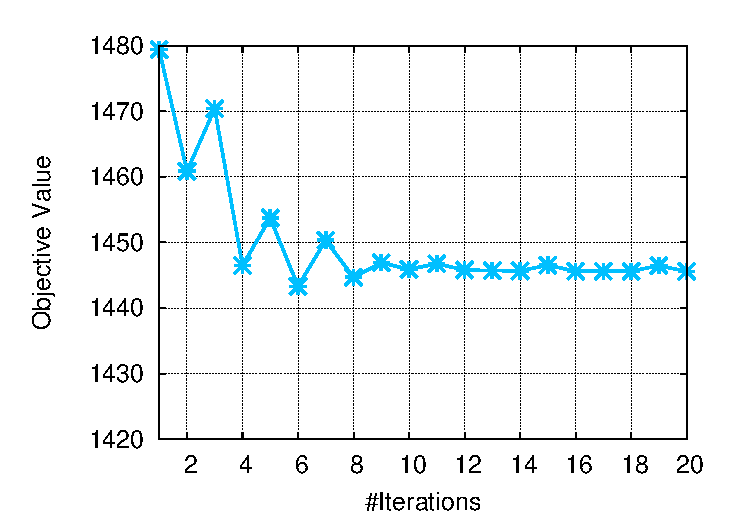
\includegraphics[width=2.8in]{figures/a1a_cnvrgnc.eps}
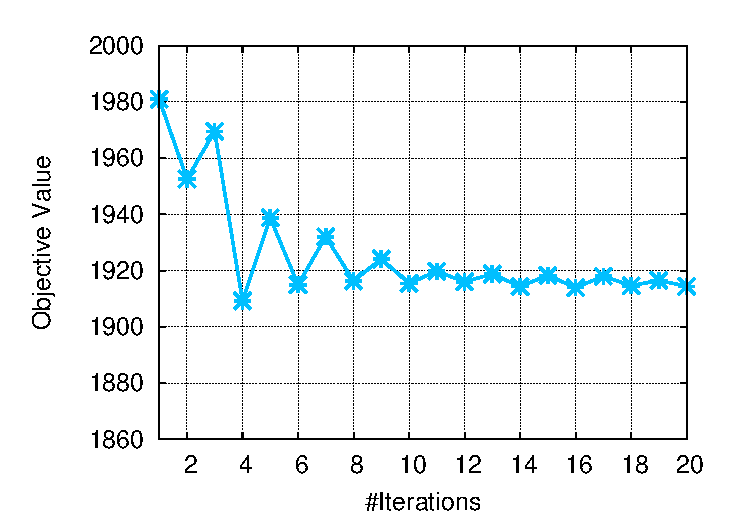
\includegraphics[width=2.8in]{figures/a2a_cnvrgnc.eps}
{\footnotesize\makebox[1.8in]{(a)~A1a}~~~~~~~~~~~~~~~~~~~~~~~~~~~~~~~~~~~~~~~~~\makebox[1.3in]{(b)~A2a}}
%\vspace{-0.1in}
\caption{Convergence of SimpleNPKL using square
hinge loss on {\em A1a} and {\em A2a}.
The parameters are $C=1$, $B=N$.} \label{fig:convergence}
\end{center}
\vskip -0.1in
\end{figure}

\subsection{Scalability Study on Adult Data Set}

In this Section, we evaluate our SimpleNPKL algorithms on another larger data set to
examine the efficiency and scalability. We adopt the {\em Adult} database, which is
available at the website of
LibSVM.\footnote{LibSVM can be found at \url{http://www.csie.ntu.edu.tw/cjlin/libsvmtools/datasets/}.} The
database has a series of partitions: A1a, A2a, $\cdots$, A5a (see Table
\ref{table:adult-set}). Since the training time complexity of NPKL using standard
SDP solvers is $O(N^{6.5})$, which cannot be applied on this database for
comparison. We only report the results of both $k$-means and constrained $k$-means clustering as the baseline
comparison.

Table \ref{table:adult} shows the clustering performance and CPU time cost (the
clustering time was excluded) of SimpleNPKL on the {\it Adult} database. From the
results, we can draw several observations. First of all, we can see that by learning
better kernels from pairwise constraints, both SimpleNPKL algorithms produce better
clustering performance than that of $k$-means clustering and constrained $k$-means clustering methods using Euclidean metric. Further, comparing
the two algorithms themselves, in terms of clustering accuracy, they perform quite
comparably, in which SimpleNPKL+SHL outperforms slightly. However, in terms of
CPU time cost, SimpleNPKL+LL with linear loss is considerably lower than
SimpleNPKL+SHL using square hinge loss.

We also plot the objective value $\J(K_,\ba)$ of SimpleNPKL on two data sets {\em
A1a} and {\em A2a} in Figure~\ref{fig:convergence}. We observe that SimpleNPKL
with square hinge loss often converges quickly within 10 iterations. Similar results can
be observed from the other data sets.

\subsection{Comparisons on Constraint Selection}

In this Section, we study the active constraint selection scheme for SimpleNPKL. Figure~\ref{fig:active-cnst-slctn} shows the clustering
performance of active constraint selection by the approach described in Section \ref{sec:cnstrnt_slctn}.

Several observations can be drawn from the results: 1) Comparing with the original approach using all constraints, the computation time is reduced by choosing a small amount of pairwise constraints. This is because the Lanczos algorithm can perform the sparse eigen-decomposition faster on a sparse matrix with fewer nonzero entries; 2) Though the active constraint selection costs more time than random selection, the former usually achieves better clustering (accuracy) performance than the latter with the same amount of constraints; 3) Using the proposed active constraint selection method to choose about half of the pairwise constraints for SimpleNPKL can often produce comparable or even better clustering performance than that using all constraints.

\begin{figure}[htbp]
%\vskip 0.2in
\begin{center}
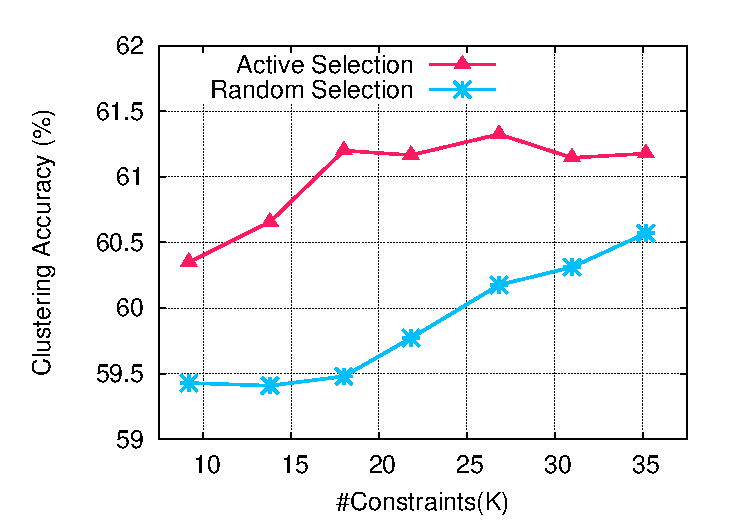
\includegraphics[width=2.8in]{figures/cnst_acc.eps}
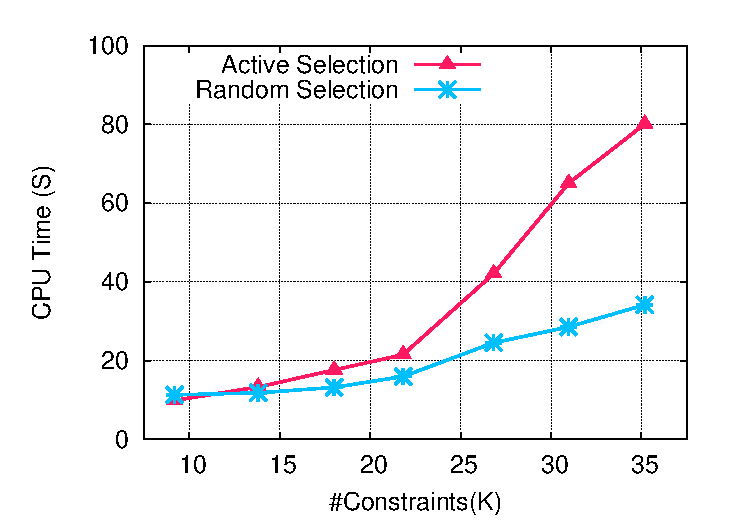
\includegraphics[width=2.8in]{figures/cnst_time.eps}
{\footnotesize\makebox[1.8in]{(a)~Clustering
Accuracy}~~~~~~~~~~~~~~~~~~~~~~~~~~~~~~~~~~~~~~~~\makebox[1.3in]{(b)~CPU Time }} \vspace{-0.1in}
\caption{Comparisons of clustering accuracy and CPU time by active
constraint selection and random selection (constraint selection time
is included) on A1a with parameters: $B=N, C=1, k=20,r=0.6$. Using
all $3.9K$ constraints directly, the accuracy is $60.8\pm2.9$ and
the CPU time is $81.6$ seconds.} \label{fig:active-cnst-slctn}
\end{center}
%\vskip -0.2in
\end{figure}

\subsection{Evaluations on Data Embedding Applications}

In this Section, we evaluate the performance of the proposed SimpleNPKL algorithms
with applications to speed up three data embedding techniques, that is, CMVU, MVE,
and SPE, respectively. Our goal is to show that SimpleNPKL is capable of producing
similar empirical results to the baseline counterpart with significant efficiency gain.
All the data sets are publicly available in the UCI machine learning repository. In all
the experiments, we simply fix $C=1$ for all the three methods, and set $B = m\times
N$, $m\in\{0.1, 1, 2, 10\}$.

\subsubsection{Colored Maximum Variance Unfolding}

The first experiment is to examine the efficiency by applying the proposed SimpleNPKL technique to solve the CMVU problem.
In particular, we examine the CMVU task for learning low-dimensional embedding on three data sets which were used in \cite{nips/SongSBG07}. Two approaches are compared:\vspace{-0.1in}
\begin{itemize}
\item {\bf CMVU}: An approximate efficient method employed by \cite{nips/SongSBG07}. Suppose $\K = \V\A\V'$, where $\V$ (of size $n \times d$, $d < n$) is fixed to be the bottom $d$ eigenvectors of the graph Laplacian of the neighborhood graph via $\mathcal N$. Thus the number of variables is reduced from $n^2$ to $d^2$.  \vspace{-0.1in}
\item {\bf CMVU+NPKL}: Our SimpleNPKL method introduced in Section \ref{sec:cmvu}. Unlike the above CMVU algorithm by approximation, our method is able to obtain the global optimal solution using the SimpleNPKL scheme without approximation.\vspace{-0.1in}
\end{itemize}

Figure \ref{fig:cmvu-senate}, \ref{fig:cmvu-news20} and \ref{fig:cmvu-usps} show the experimental results of visualizing the embedding results in a 2D space and the CPU time cost of CMVU. The time costs of CMVU+NPKL were also indicated in the captions of those figures.
As we can observe from the visualization results, the proposed CMVU+NPKL is able to produce comparable embedding results as those by the original CMVU in most cases. Further, by examining the time cost, we found that the time cost of CMVU increases with dimensionality $d$ exponentially due to the intensive computational cost of solving the SDP problem. In contrast, the proposed CMVU+NPKL is able to find the global optima efficiently, which is much faster than CMVU when $d$ is large. Although CMVU could be faster than CMVU+NPKL for very small $d$ values, it is important to note that the optimal $d$ value is often unknown for many applications. The proposed CMVU+NPKL approach can efficiently and directly resolve the CMVU problem without soliciting the approximation step.\vspace{-0.1in}


\begin{figure}[htpb]
%\vskip 0.2in
\begin{center}
\subfigure[Time cost of CMVU with the rank.]
{
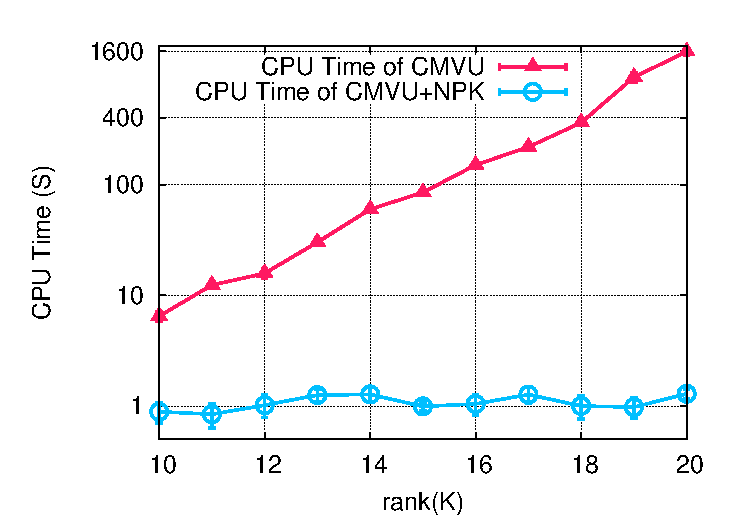
\includegraphics[width=2.0in]{figures/cmvu_time_senate.eps}
}
\subfigure[Embedding of CMVU.]
{
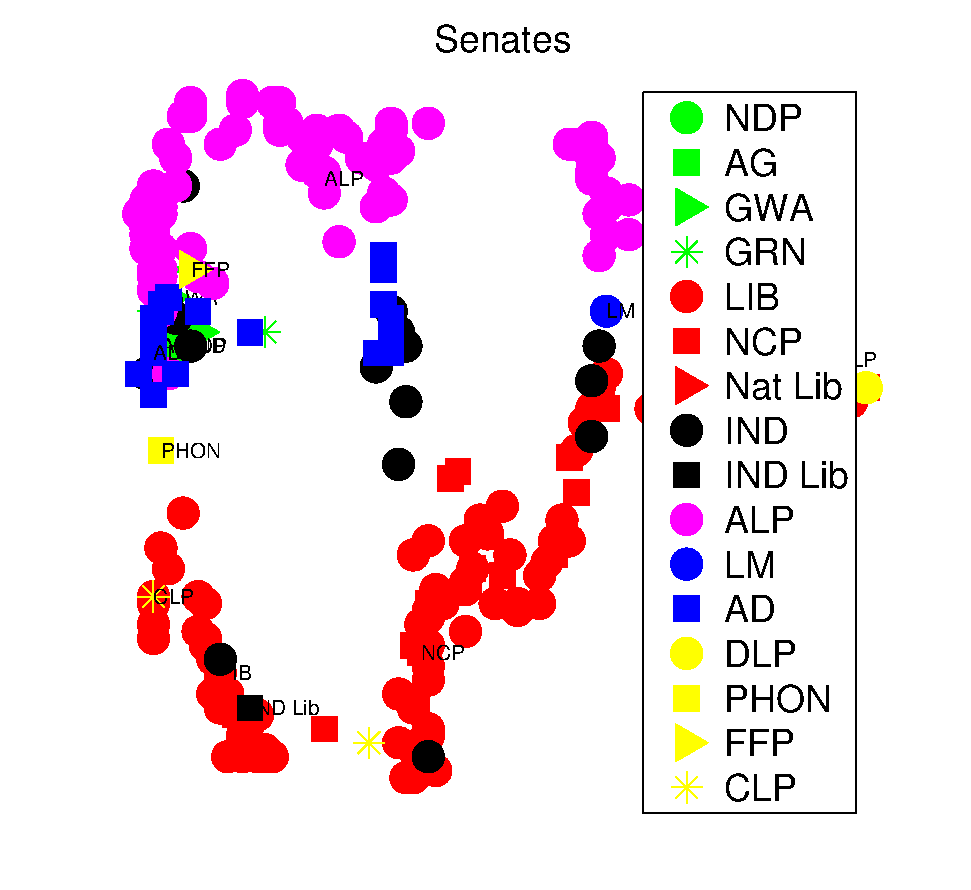
\includegraphics[width=1.8in]{figures/senate_cmvu.eps}
}
\subfigure[Embedding of CMVU+NPKL.]
{
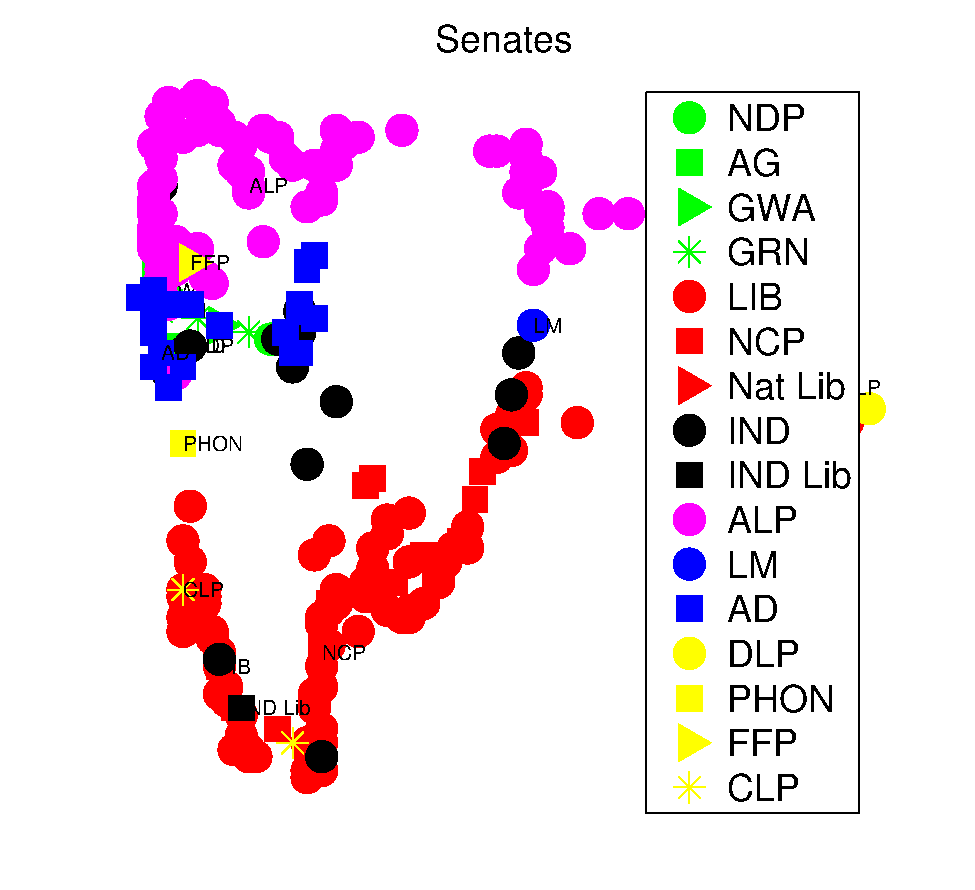
\includegraphics[width=1.8in]{figures/senate_cmvu_npk.eps}
}\vspace{-0.1in}
\caption{Comparisons of CMVU and CMVU+NPKL on {\em senate} data set. \textbf{Time cost of CMVU+NPK is $1.50\pm0.06$ seconds.} } \label{fig:cmvu-senate}\vspace{-0.1in}
\end{center}
%\vskip -0.2in
\end{figure}

\begin{figure}[!h]
%\vskip 0.2in
\begin{center}
\subfigure[Time cost of CMVU with the rank.]
{
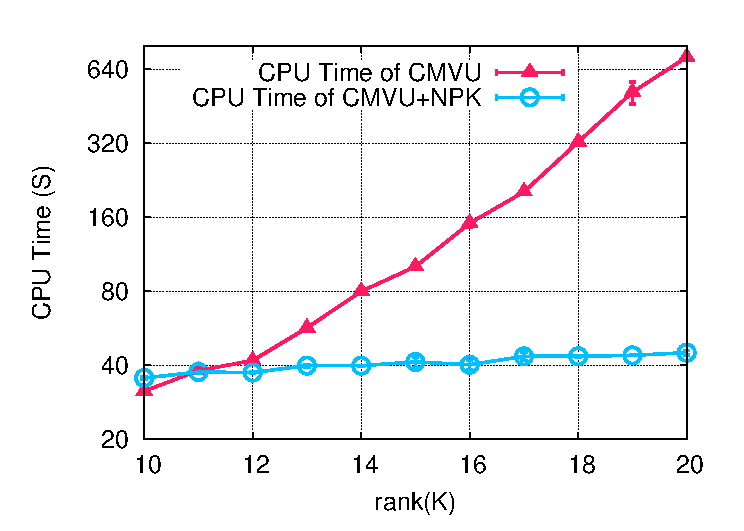
\includegraphics[width=2.0in]{figures/cmvu_time_news20.eps}
}
\subfigure[Embedding of CMVU.]
{
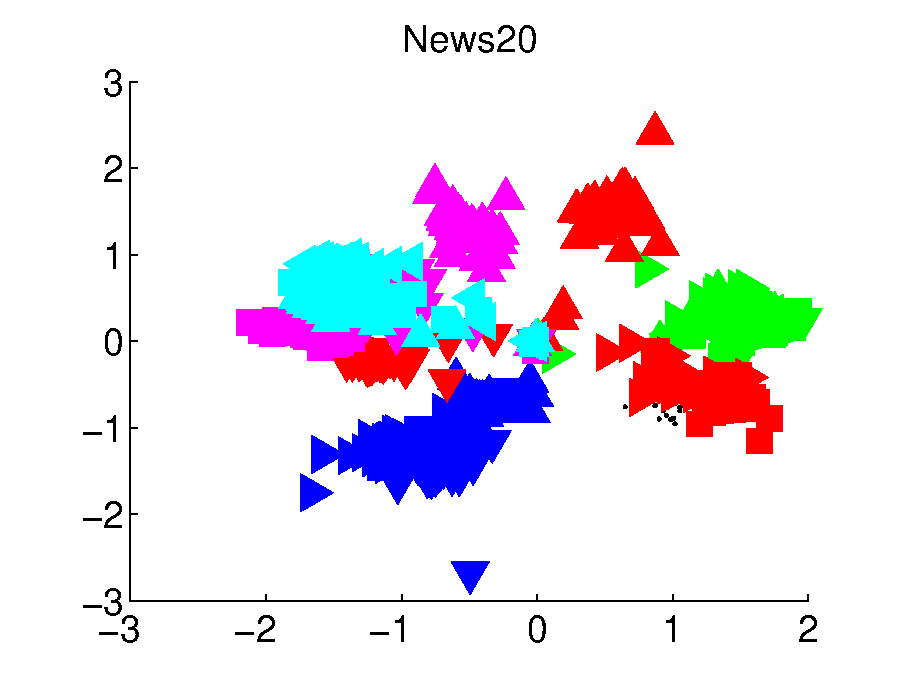
\includegraphics[width=1.8in]{figures/news20_cmvu.eps}
}
\subfigure[Embedding of CMVU+NPKL.]
{
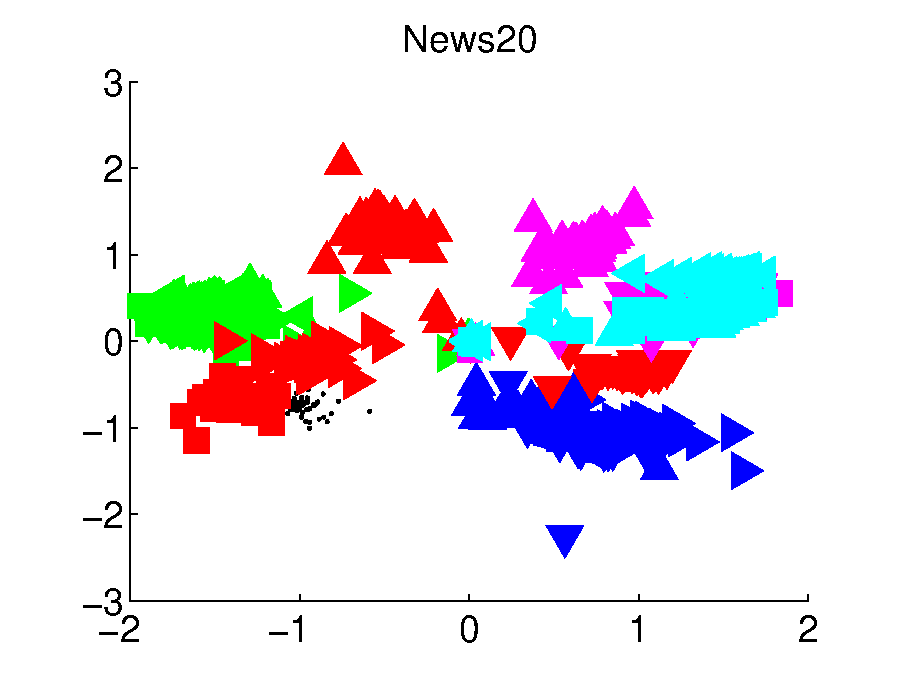
\includegraphics[width=1.8in]{figures/news20_cmvu_npk.eps}
}
\caption{Comparisons of CMVU and CMVU+NPK on {\em news20} data set. \textbf{Time cost of CMVU+NPKL is $120.4
\pm1.7$ seconds.} } \label{fig:cmvu-news20}\vspace{-0.1in}
\end{center}
%\vskip -0.2in
\end{figure}

\begin{figure}[!htbp]
%\vskip 0.2in
\begin{center}
\subfigure[Time cost of CMVU with the rank.]
{
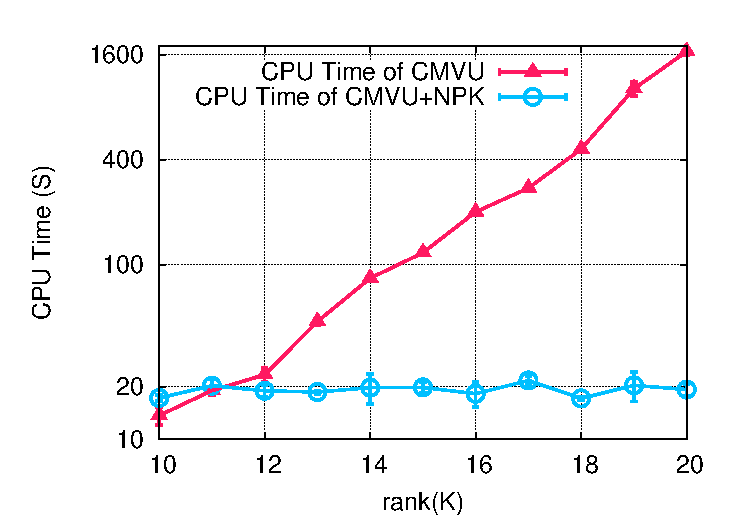
\includegraphics[width=2.0in]{figures/cmvu_time_usps.eps}
}
\subfigure[Embedding of CMVU.]
{
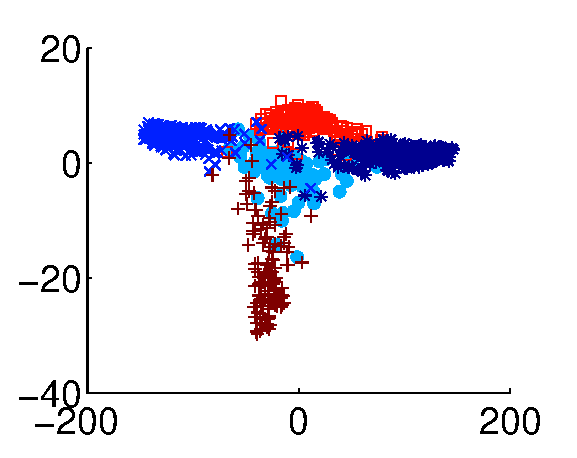
\includegraphics[width=1.8in]{figures/usps_cmvu_d20.eps}
}
\subfigure[Embedding of CMVU+NPKL.]
{
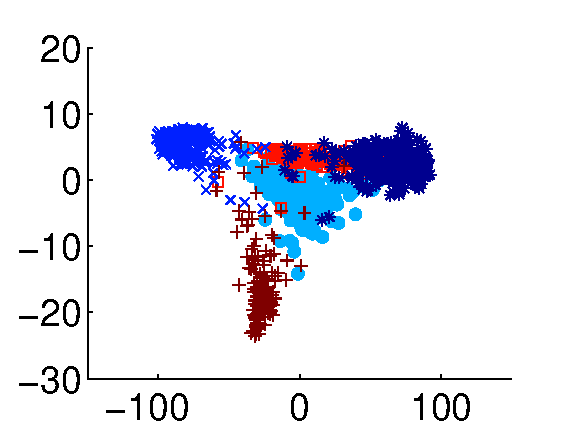
\includegraphics[width=1.8in]{figures/usps_cmvu_npk.eps}
}
\caption{Comparisons of CMVU and CMVU+NPKL on {\em usps} data set. \textbf{Time cost of CMVU+NPKL is $28.95\pm1.8$ seconds.} } \label{fig:cmvu-usps}\vspace{-0.1in}
\end{center}
%\vskip -0.2in
\end{figure}


\subsubsection{Minimum Volume Embedding and Structure Preserving Embedding}

This experiment is to examine the embedding performance of the SimpleNPKL technique with applications to MVE \cite{aistats/ShawJ07} and SPE \cite{icml/ShawJ09} tasks. In particular, five approaches are compared:%\vspace{-0.1in}
\begin{itemize}
  \item {\bf KPCA}: The classical Kernel Principle Component Analysis algorithm;\vspace{-0.1in}
  \item {\bf MVE}:  The algorithm summarized in Table 1 in \cite{aistats/ShawJ07}. Pay attention to the SDP solver in Step 5 and 6, which is the key for the success of MVE.  \vspace{-0.1in}
  \item {\bf MVE+NPKL}: The embedding algorithm based on our SimpleNPKL algorithm. Refer to Section \ref{sec:mve} for detailed discussion.\vspace{-0.1in}
  \item {\bf SPE}: The algorithm summarized in Table 1 of \cite{icml/ShawJ09}.   \vspace{-0.1in}
  \item {\bf SPE+NPKL}: The embedding algorithm based on the proposed SimpleNPKL algorithm. Refer to Section \ref{sec:spe};
\end{itemize}
To examine the embedding results quantitatively, we follow the previous studies \cite{aistats/ShawJ07,icml/ShawJ09} to evaluate the classification performance on the embedding data by performing k-nearest neighbor classification. Similar to the settings in \cite{icml/ShawJ09}, we randomly choose 100 points from the largest two classes for each data set, and then divide the data examples into training/validation/test sets at the ratios of 60:20:20. The validation set is used to find the best parameter of $k$ for $k$-NN classification.


Table~\ref{table:knn-embedding-acc} shows the comparison of the classification results by five different approaches. From the results, we can see that the two proposed algorithms, MVE+NPKL and SPE+NPKL, are generally able to achieve the competitive classification results that are comparable to the other two original algorithms using a standard SDP solver. Among all compared algorithms, MVE+NPKL tends to achieve slightly better performance than the other approaches. All these results show that the proposed algorithms are effective to produce comparable embedding performance.


\begin{table*}[!hptb]
\centering
%\hspace{-0.1in}
\begin{center}
%\begin{small}
\begin{tabular}{c | r | r r| r r }
\hline
Data Set    & KPCA &MVE &MVE+NPKL &SPE &SPE+NPKL \\

\hline
Wine   &90.5 $\pm$5.6 &{\bf 91.9 $\pm$6.6} &90.9$\pm$5.8   &75.2 $\pm$0.09  &87.1 $\pm$7.9\\

Ionosphere    &79.8$ \pm$7.3   &{\bf 86.3 $\pm$7.3}   &84.2$\pm$8.5   &80.4 $\pm$10.4    &83.6 $\pm$7.8\\

Heart    &{\bf 65.6 $\pm$8.4} &62.4 $\pm$9.8   &62.9 $\pm$9.8   &54.9 $\pm$10.2   &62.2 $\pm$11.1\\

Sonar    &58.2 $\pm$12.4   &59.2 $\pm$10.2   &{\bf 59.8 $\pm$12.2}   &57.4 $\pm$11.1   &59.4 $\pm$11.4\\

Glass     &70.7 $\pm$9.8    &73.5 $\pm$7.8    &{\bf 74.5 $\pm$10.4}  &61.7 $\pm$9.7  &69.4 $\pm$8.7\\

Spiral   &98.7 $\pm$2.4 &69.1 $\pm$9.8 &{\bf 98.8 $\pm$2.4} &76.7 $\pm$0.07 &82.9 $\pm$8.4\\

Australian   &63.2 $\pm$9.8   &61.3 $\pm$8.2 &{\bf 63.8 $\pm$9.3} &60.1 $\pm$ 0.10 &59.5 $\pm$10.1\\

Breast cancer   &91.9 $\pm$5.4 &92.9 $\pm$4.6 &92.4 $\pm$5.8 &93.4 $\pm$0.07 &{\bf 94.4 $\pm$5.5}\\

\hline
\end{tabular}
%\end{small}
\end{center}%\vspace{-0.2in}
\caption{$k$-NN classification accuracy on the 2D embedded results. (The best results are bolded.)}
\label{table:knn-embedding-acc}
\end{table*}



Next we compare the computational cost of the proposed algorithms against their original methods, respectively. Table~\ref{table:knn-embedding-time} shows the summary of average CPU time cost of the compared algorithms. From the results, it is clear to see that the two proposed algorithms, MVE+NPKL and SPE+NPKL, are significantly more efficient than the other two original algorithms, respectively. By comparing MVE and MVE+NPKL, we found that MVE+NPKL achieves about $10$ to $30$ times speedups over the original MVE algorithm; the speedup values are even more significant for the SPE problem, where the proposed SPE+NPKL algorithm attains about $50$ to $90$ times speedup over the original SPE algorithm. These promising results again validate the proposed SimpleNPKL is effective for improving the efficiency and scalability of the three data embedding tasks.


\begin{table*}[!hptb]
\centering
%\hspace{-0.1in}
\begin{center}
\begin{small}
\begin{tabular}{c | r r r| r r r }
\hline
Data Set &MVE &MVE+NPKL &\!\!SpeedUp &SPE &SPE+NPKL &\!\!SpeedUp\\

\hline
Wine &2.92 $\pm$0.06 &{\bf 0.34 $\pm$0.04} &8.5   &47.72 $\pm$0.29 &0.51 $\pm$0.01 &93.6\\

Ionosphere &16.98 $\pm$0.16  &1.14 $\pm$0.01 &14.9  &30.07 $\pm$1.25  &{\bf 0.60 $\pm$0.01} &50.1\\

Heart &9.64 $\pm$0.00 &{\bf 0.38 $\pm$0.02}   &25.3 &48.18 $\pm$0.31  &0.51 $\pm$0.11 &94.5\\

Sonar   &7.50 $\pm$0.13   &{\bf 0.46 $\pm$0.01}   &16.3   &30.40 $\pm$1.16 &0.61 $\pm$0.02 &49.8 \\

Glass &11.08 $\pm$0.26    &{\bf 0.39 $\pm$0.01}    &28.2  &29.10 $\pm$0.12   &0.53 $\pm$0.01   &54.9\\

Spiral &18.28 $\pm$0.28 &{\bf 0.46 $\pm$0.00} &39.7 &47.91 $\pm$0.91 &0.48 $\pm$0.01  &99.8\\

Australian &4.61 $\pm$0.03   &{\bf 0.30 $\pm$0.02} &15.4 &28.94 $\pm$0.11 &0.53 $\pm$0.01 &54.6\\

\!\!\!Breast cancer\!\! &16.59 $\pm$0.10 &{\bf 0.49 $\pm$0.02} &33.9 &48.72 $\pm$0.26 &0.56 $\pm$0.01 &87.0\\

\hline
\end{tabular}
\end{small}
\end{center}%\vspace{-0.2in}
\caption{The evaluation of CPU time cost of different algorithms and the speedup of the SimpleNPKL method over the standard SDP solver. (The best results are bolded.)}
\label{table:knn-embedding-time}
\end{table*}

To further illustrate the scalability of SPE+NPKL, we propose to solve a real-world embedding task on a large data set. In particular, we crawled a Flickr\footnote{Flickr can be found at \url{http://www.flickr.com/}.} data set, which consists of 3,660 Flickr user profiles and a collection of 3.7 million photos uploaded by these users. Each photo was annotated with a set of textual tags by users. Accordingly the photos for a particular Flickr user are described by tiling these tags. In total, our data set has 359,832 tags and 93,692 unique tags. Each Flickr user has a contact list, which is a collection of Flickr users who may share similar tastes / interests in their photo sharing. In our data set, every user has 19.1 contacts on average. We thus set $|\mathcal N|$ to 20 in both MVE and SPE. Moreover, there are $97,212$ interest groups, and each Flickr user could belong to one or more interest groups. We compute {\em tf-idf} weight for the tags to represent a Flickr user (here the document frequency for a tag is actually the number of users annotated with that tag, that is, one or more photos of this user annotated with the tag). The k-nearest neighbor graph for MVE is constructed using cosine similarity between Flickr users. For SPE, we further constrain that the intra-group distance is smaller than the inter-group distance. In general, people who are friends or similar to each other tend to join the same interest group. Our goal is to apply the proposed MVE+NPKL and SPE+NPKL algorithms on these Flickr users in order to draw the 2D embedding results of the Flickr users exclusively belonging to two different interest groups: {\em B\&W}\footnote{{\em B\&W} can be found at \url{http://www.flickr.com/groups/blackwhite/}.} and {\em Catchy Colors}\footnote{{\em Catchy Colors} can be found at \url{http://www.flickr.com/groups/catchy/}.} as shown in Figure 7.

\begin{figure}[h]
%\hspace{-10cm}
\begin{center}
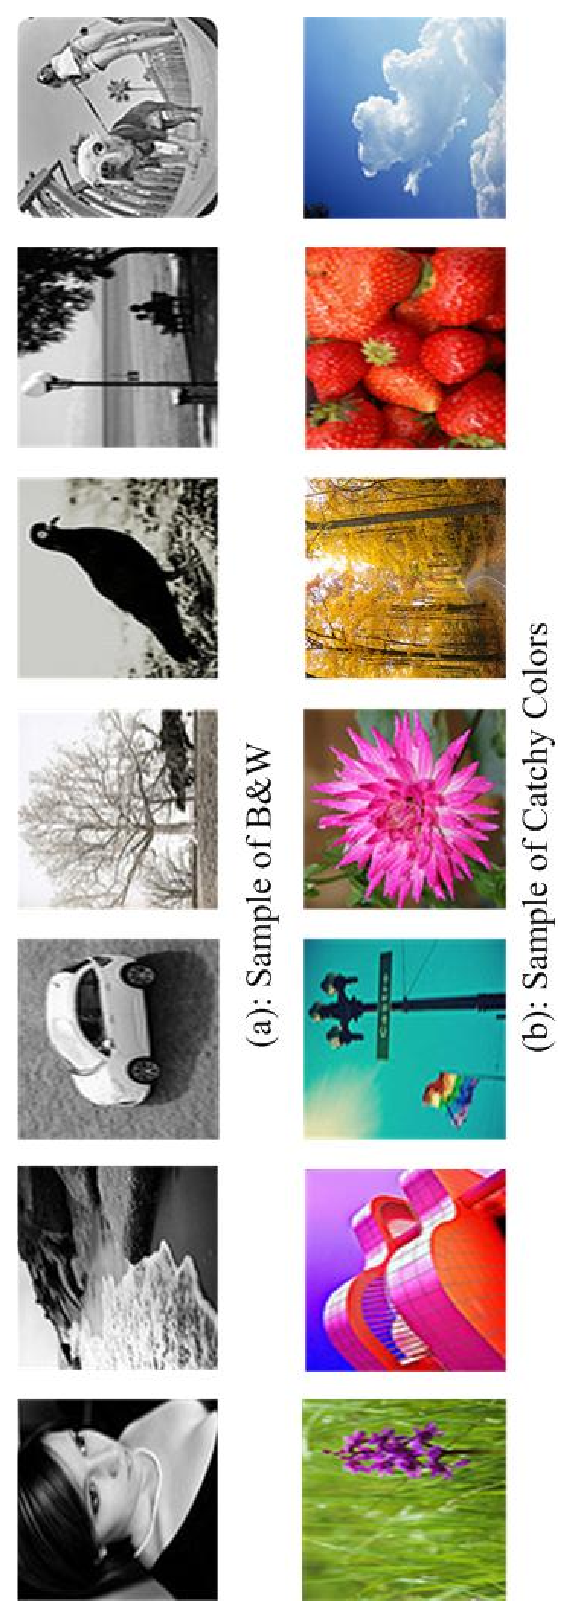
\includegraphics[width=2.0in,angle=270]{figures/sample.eps}%\hspace{-10cm}
\caption{Sample photos from two Flickr interest groups: {\em B\&W} and {\em Catchy Colors}.}
\end{center}
\end{figure}

\begin{figure}[htbp]
%\vskip 0.2in
\begin{center}
\subfigure[MVE+NPKL]{
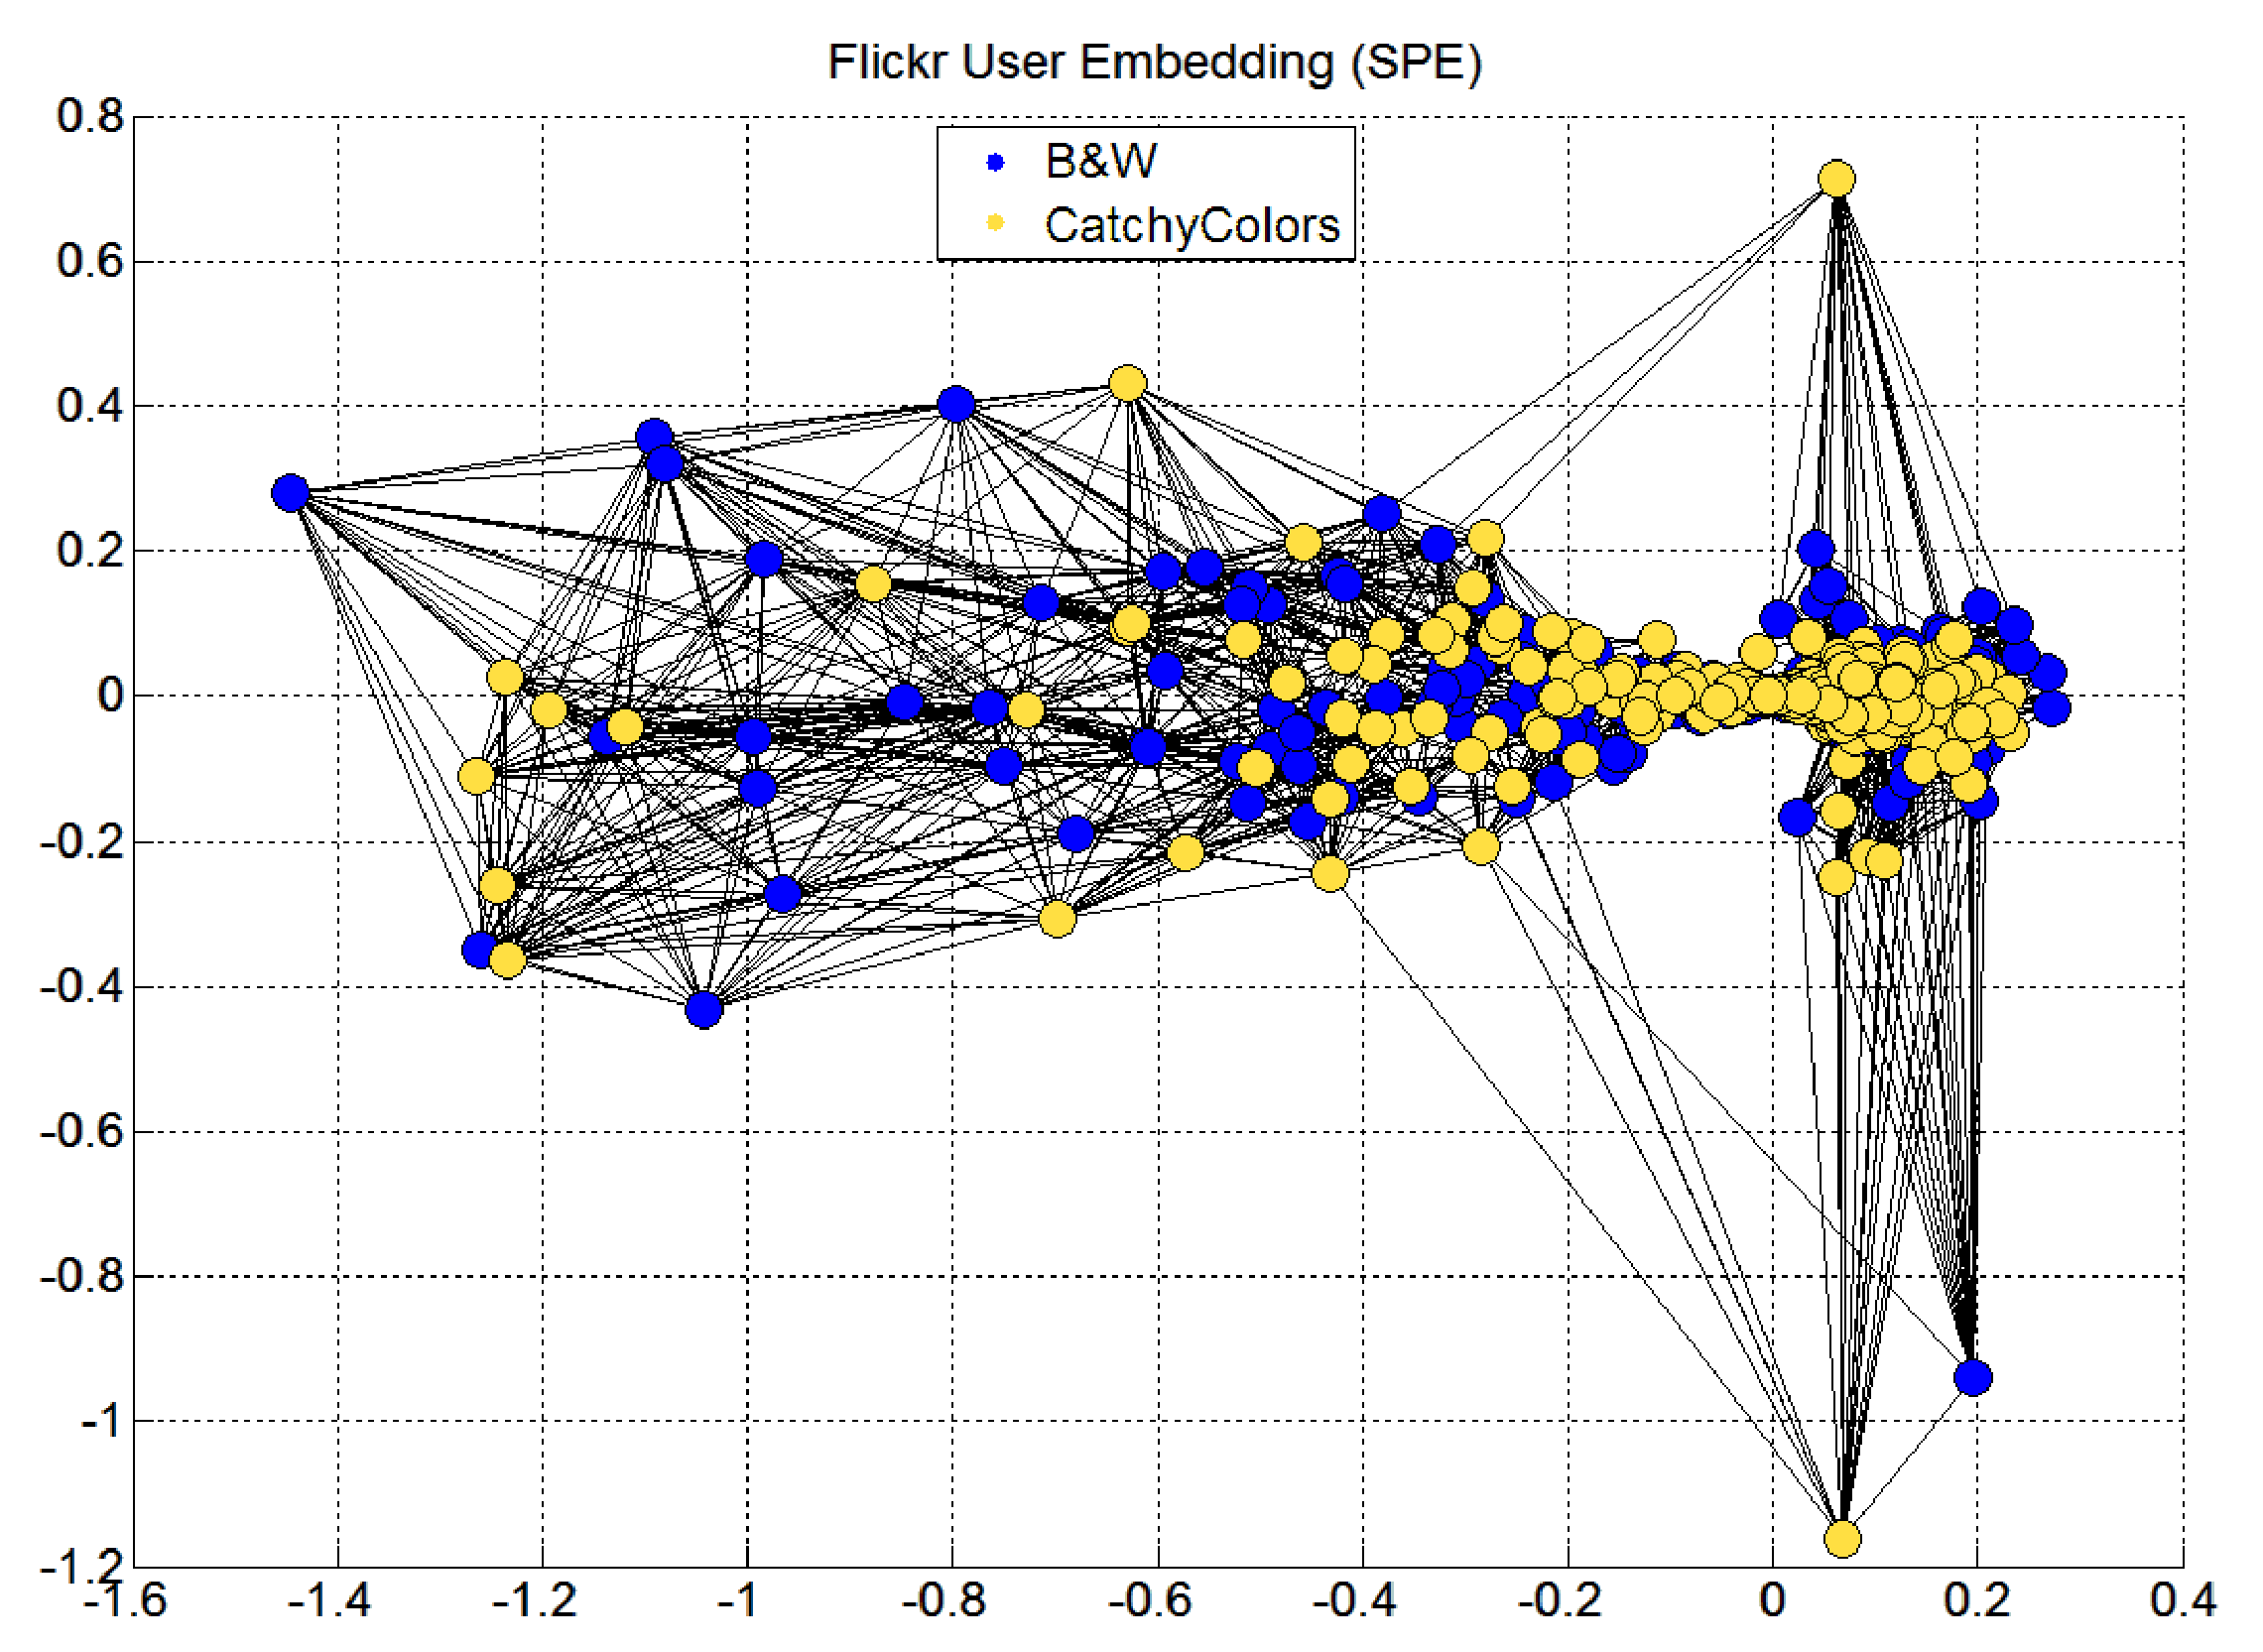
\includegraphics[width=5.5in,height=8cm]{figures/mve.eps}
}
\subfigure[SPE+NPKL]{
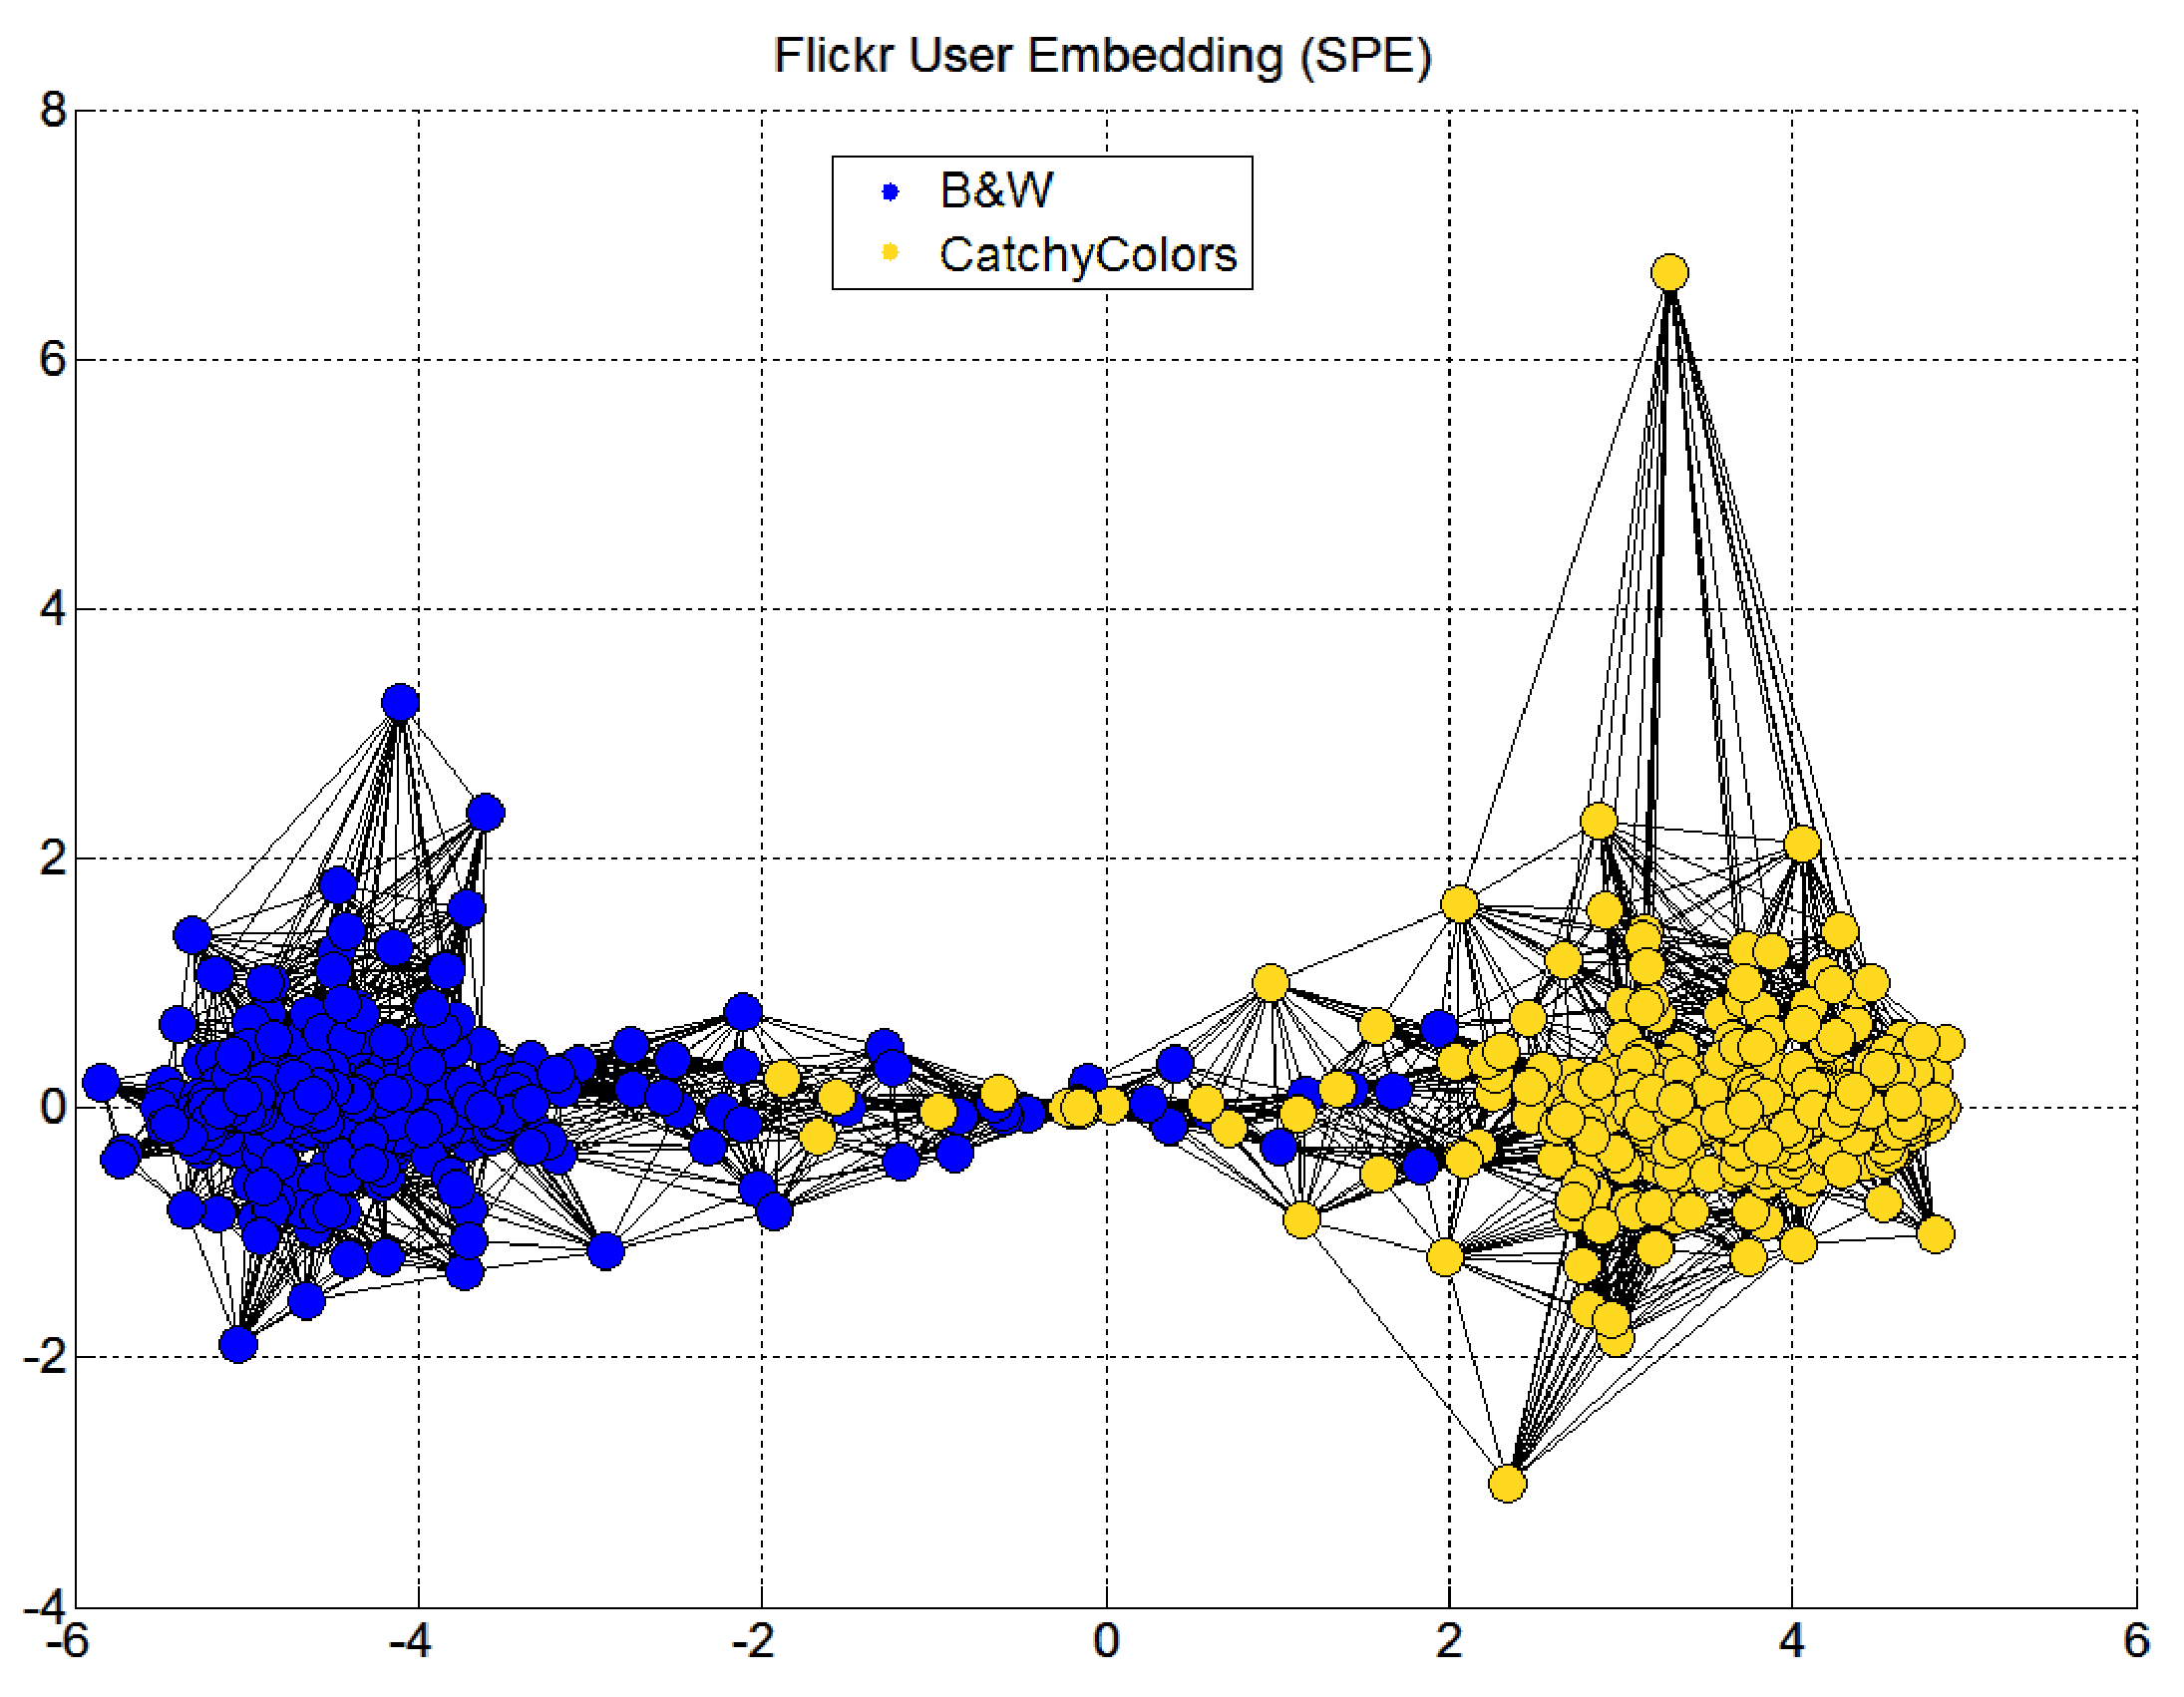
\includegraphics[width=5.5in,height=8cm]{figures/flickr.eps}
}
\caption{The 2D embedding result of Flickr users exclusively belonging to the interest group {\em B\&W} (blue points) and  {\em Catchy Colors} (red points). The CPU time cost of MVE+NPKL and SPE+NPKL are 27.2 minutes and 196.4 minutes, respectively. } \label{fig:flickr}
\end{center}
%\vskip -0.2in
\end{figure}

Specifically, the theme of the group B\&W is related to a collection of photos with black and white color only. The corresponding top 5 annotated tags for B\&W are $\{${\em bw, black and white, black, white, portrait}$\}$. In contrast, the top 5 tags for CatchyColors include $\{${\em red, blue, green, flower, yellow}$\}$. Therefore, photos in the latter group are more colorful than the ones in B\&W. An illustration of photos belonging to these two groups are depicted in Figure 6. However, the semantics of photos of these two groups are highly overlapping. Accordingly, the embedding results of MVE are highly overlapped as shown in Figure 7 (a), though it drives the spectral information into the top eigenvectors of the learned kernel matrix. On the other hand, by constraining intra-group distance less that inter-group distance, SPE can preserve the topology structure of these two groups as shown in Figure 7 (b). The 2D embedding shows the cluster structure rather clearly.

Note that the original algorithms using general SDP solvers cannot directly apply on the above large real data set. The proposed SimpleNPKL framework makes it feasible to analyze the emerging social networking problems using kernel learning methods. We hope our preliminary attempt in this chapter could shed a light on a series of important applications in the future, including: 1) {\bf Visualization:} as illustrated in Figure 7, we are able to obtain an intuitive understanding about the distribution of the entities in a social networking community. From Figure 7 (b), one can also observe the abnormal entities (e.g., the red dot on the right upper corner) and prototypes (the ones located at the centers of clusters). This may also benefit spam user detection and important user identification applications;  2) {\bf Friend suggestion:} Given a Flickr user $U_i$, we can rank the other users $U_j$ according to their similarity to $U_i$ computed by the learned non-parametric kernel $K_{ij}$. With such information, a user can quickly find the other users of similar interests/tastes in photo sharing so as to facilitate the social communication between the users; 3) {\bf Interest group recommendation:} It is interesting and beneficial to develop an intelligent scheme for recommending a Flickr user some interest groups. By applying the proposed kernel learning techniques to find similarity between Flickr users, it is possible for us to develop some recommendation scheme that suggests a Flickr user some interest groups that received the highest numbers of votes from its neighbors.


%==================================================
\section{Summary}\label{sec:con}
%==================================================

In this chapter, we investigated a family of SimpleNPKL algorithms for improving the efficiency and scalability of the Non-Parametric Kernel Learning (NPKL) from large sets of pairwise constraints. We demonstrated that the proposed
SimpleNPKL algorithm with linear loss for the pairwise constraints enjoys a closed-form solution, which can be simply computed by efficient sparse eigen-decomposition, such as the Lanczos algorithm. Moreover, our
SimpleNPKL algorithm using other loss functions (including square hinge loss, hinge loss, and square loss) can be transformed into a saddle-point minimax optimization problem, which can be solved by an efficient iterative optimization procedure that only involves sparse
eigen-decomposition computation. In contrast to the previous standard SDP solution, empirical results show that our approach achieved the same/comparable accuracy, but is significantly more efficient and scalable for large-scale data sets. We also explore some active constraint selection scheme to reduce the pairwise constraints in SimpleNPKL, which can further improve both computational efficiency and the clustering performance. Finally, we also demonstrate that the proposed family of SimpleNPKL algorithms can be applicable to other similar machine learning problems, in which we studied three example applications on data embedding problems. In the future, we will extend our technique for solving other SDP related machine learning problems. 